%!TEX root = ../thesis_a4.tex

\chapter{Melodic pattern processing: similarity, discovery and characterization}
\label{chap:melodic_pattern_processing}

\section{Introduction}
\label{sec:patterns_introduction}

In this chapter we present our proposed methodology for processing patterns in melodies of \gls{iam}. We describe our approach for discovering melodic patterns in large audio music collections, evaluate a number of melodic similarity measures, propose ways to improve melodic similarity computation in \gls{iam}, and finally, present an approach to characterize the discovered melodic patterns. The description provided in this chapter is primarily based on our work presented in~\cite{gulati_SITIS_2014,gulati_ICASSP2015, gulati_ISMIR_2015,gulati_communities_2016}. %regarding evaluation of melodic similarity measures, in~\cite{gulati_ISMIR_2015} about utilizing culture specific melodic characteristics to improve similarity, in~\cite{gulati_SITIS_2014} about methodology to mine melodic patterns in sizable audio collections of \gls{iam}, and finally, in~\cite{gulati_communities_2016} about characterization of the discovered melodic patterns. 

\TODO{In this introduction, relate what we did to existing approaches and what exists and contrast a bit, somehow}

One of the key objectives of this dissertation is to extract melodic patterns in sizable audio collections of \gls{iam}. These patterns can then be characterized and used for performing computational tasks such as \gls{raga} recognition~(\chapref{chap:raga_recognition}). From the literature review presented in~\chapref{chap:background} we see that the approaches for extracting patterns in time-series data can be broadly put into two categories (\figref{fig:types_of_methodologies_for_extraction}). Notice that these are also the two types of paradigms used in machine learning. One of the types of approaches are supervised in nature, wherein a system knows a priori the kind of patterns to be extracted. The system is fed with example patterns and is expected to extract all their occurrences in the data. In the context of our task, this would mean that musicians would provide us with example melodic patterns, using which we then aim to retrieve all their occurrences in an audio collection. This kind of an approach is frequently taken for a query based retrieval systems such as in query by humming or in cover song detection\TODO{ref, are these tasks valid in this context?}. 


\begin{figure}
	\begin{center}
		
\includegraphics[width=\figSizeSixty]{ch06_patterns/figures/figure_todo.pdf}
	\end{center}
	\caption{Two types of approaches for pattern extraction in time-series data.}
	\label{fig:types_of_methodologies_for_extraction}
\end{figure}

Another type of approaches are unsupervised in nature (\figref{fig:types_of_methodologies_for_extraction}), wherein a system tries to discover patterns in a collection of data without any training examples from an expert or a query. In the context of melodic pattern discovery, such a system will not require any input from musicians in terms of annotated examples of melodic patterns. The patterns are discovered from the data itself. This brings us to an interesting question, what do we mean by a melodic pattern given we do not have any example of it provided by an expert? Recall (Section XX), in the scope of this dissertation any recurring melodic fragment is considered as a melodic pattern. We assume that since it repeats, its not by coincidence and that it has some meaning since the artist rendered the exact fragment again\TODO{rephrase}. It should be noted that by recurrence or repetition we do not mean the numerical repetition of the time-series (pitch fragment) data, we mean the musical recurrence of the melodic pattern, which might undergo melodic variations allowed in the music tradition without loosing its musical identity. In addition, the scope of our definition is only recurring melodic patterns which we carefully differentiate from melodic phrases or melodic motifs, wherein the latter have a musical significance attached to them.

In this dissertation we follow an unsupervised approach for discovering melodic patterns in sizable audio collections of \gls{iam}. Our key motivation behind an unsupervised approach is that it does not require any annotated data, i.e. example melodic patterns. The main reasons why we prefer to work without examples given by musicians are as follows (written very very roughly): \TODO{write these in paragraphs, in points they look very prominent and like bold statements}
\begin{itemize}
	\item The system will not be biased by the examples given by musicians. Selecting patterns that are musically meaningful involves a subjective decision. It is not guaranteed that musicians agree to the same set of melodic patterns. By following an unsupervised approach we can avoid this bias and can discover all types of repeating patterns, which later we can characterize.
	\item There is a fair possibility of discovering novel melodic patterns that musicians might not consciously pay attention to. 
	\item In \gls{iam} which is fundamentally improvisatory in nature, where the improvisation to a large extend is based around melodic patterns, annotating comprehensively each and every short repeating fragment of melody is virtually impossible.
	\item Not that the annotation process is tedious but it might also be ill an defined task. Several times despite a melodic pattern is said to be inspired by another pattern, not necessarily a repetition of that. In such cases it becomes difficult to annotate comprehensive all the melodic patterns. 
	\item Humans have a limited memory, thus a phrase occurring after several minutes in a performance might not be identified as a repeating patterns. We found that when we ask musicians to mark patterns, they do not have repetition as the idea for marking patterns. Instead they from their learning of characteristic melodic patterns mark on the ones which they remember are characteristics of the \gls{raga}.
	\item Another limitation of the  human listener we observed is segmentation. We found tha several times musicians miss marking a characteristic phrase if that occurs in a completely different melodic context in which they are use to listening it.  
\end{itemize}

\TODO{This is also an area that noone ever has worked with, there is no such an approach for indian art music. In fact if you think of it not even for western music!!!. This could also go in the motivation of choosing this approach}

Along with the aforementioned advantages, there are several challenges in following an unsupervised approach for pattern extraction. One of the most challenging aspects of such approaches is its quantitative evaluation. Due to the absence of ground-truth annotations evaluating such approaches becomes difficult. For a data-driven research methodology this becomes even more complex since the system parameters are optimized based on the data. After our first study presented in~\cite{gulati_SITIS_2014} on mining melodic patterns we realized that selecting optimal values of the system parameters is notoriously difficult in a completely unsupervised setup. As a result of which we bootstrap\TODO{is it a correct word?} our methodology by first improving melodic similarity computation, one of the core processing blocks of the system in a supervised setup. We use a collection of audio recordings annotated with characteristic melodic phrases of \gls{raga} and perform a grid search to obtain optimal values of the system parameters and the most relevant similarity measure~\citep{gulati_ICASSP2015}. We further put efforts to improve the computation of melodic similarity by exploiting culture specific characteristics of melodies in Carnatic and Hindustani music~\citep{gulati_ISMIR_2015}.

There are different types of melodic patterns in melodies of \gls{iam} such as gamakas and \gls{raga} motifs (Section XX). These patterns have varied musical significance and their function role differs considerably. It is therefore essential to characterize the discovered melodic patterns in order to utilize them effectively in other computational tasks~\citep{gulati_communities_2016}. In this chapter we describe these methods in detail and elaborate our findings. Based on the type of computational task we divide this chapter into 4 different parts; in~\secref{sec:patterns_evaluation_of_similarity_measures} we present different choices for computing melodic similarity and perform a grid search to optimize system parameters, in~\secref{sec:patterns_improving_melodic_similarity} we propose an approach to improve further the computation of melodic similarity, in~\secref{sec:patterns_melodic_pattern_discovery} we outline our methodology for discovering melodic patterns in audio collections of \gls{iam}, and finally, in~\secref{sec:patterns_characterization_of_melodic_patterns} we explain our approach for characterizing the discovered melodic patterns according to their musical significance. 

 

%
%THINGS TO HAVE
%\begin{itemize}
%	\item What is lacking in state of the art? how does your work relate to that
%	\item Context of the work, how the flow of research went
%	\item introduction and motivation of the task done in the chapter
%	\item contexualization based on the state of the art
%\end{itemize}
%
%General
%\begin{itemize}
%	\item what do we call patterns, motifs, phrases etc!
%	\item What are the characteristics of Indian art music, how are they based around patterns, what are the different types of patterns in INdian art music, what is their time-scale, what kind of patterns are we interested in, what is the importance of these patterns and what can we do if we can extract these patterns.
%	\item what are the tasks that we have addressed in pattern processing of Indian art music, what is our aim, what are two kinds of approaches to process patterns (sup + unsup]), what do we follow
%	\item existing work on pattern processing, different aspects, melody representation, similarity measure, search and discovery! its important to evaluate how they work on our case. Highlight that for indian art music when this work started nothing much was done! however during the course of this dissertation there is quite a bit of work done in collaboration. 
%	\item What are the challenges in pattern processing of indian art music	
%\end{itemize}
%
%
%
%Similarity
%\begin{itemize}
%	\item how is the idea of pattern related with similarity or melodic similarity in particular,
%	\item reiterate the idea of pattern connection with similarity. What is the similarity of, time scale of patterns we are talkin about.
%	\item What are the challenges in studying similarity
%	\item what is our motivation to study similarity? core block in discovery and search, core of pattern processing. Why are we studying in section supervised way? what don't we want to use this way
%	\item how do we study and develop appraoches for measuring similarity, explain that we cast it as a retrieval task.
%	\item What has been done in state of the art? explain that there are so many different parameters, different considerations, some of them might depend on the culture dependent characteristics of a music tradition.
%	\item why have we limited ourselves to only few choices of distance measures.
%	\item declaration that choices are inspired by the limtations posed by the next block in terms of computational complexity!
%	\item Its challenging because musician's haven't marked according to repetition, they dont even compare those fragments, they compare each of them with the image they have iun their minds of the pattern. Which makes this task challenging. 
%\end{itemize}
%
%Improvement in similarity
%\begin{itemize}
%	\item What have we done in previous study
%	\item what did we leave which is covered in this study. What is the main issue that we saw? what cultural specific aspect can we exploit further
%	\item What is the advantage of taking the approach which is taken! 
%\end{itemize}
%
%Discovery
%\begin{itemize}
%	\item Reiterate two ways of going for pattern processing
%	\item Motivate why do we follow the unsupervised analysis, benefits of supervised and more than anything, limitations of unsupervised
%	\item clearly define what is our aim, what kind of patterns we want, musical quality and characteristics, length? etc
%	\item challenges in discovery, challenges in discovery with indian music, melodic representation, similarity measure etc. What have we learned from supervised anlaysis that we can take advantage of in here!!!
%	\item what is done in the sate of the art, why can't we replicate that, why do we need another method.
%	\item What can be its advantages
%	\item our initial experimnts with euclidean distance, there is high computational complecity inboleved, and a lot of procedures are limited becausue of that...entire approach ismotivated by that, present block diagram, motivate why we choose this block diagram because for the entire music collection we couldn't find any pattern in 24 hours by euclidean distance. 
%\end{itemize}

\section{Melodic Similarity: Approaches and Evaluation}
\label{sec:patterns_evaluation_of_similarity_measures}

As explained in~\secref{sec:patterns_introduction} in all our studies in this dissertation we consider repeating melodic fragments as melodic patterns. The concept of repetition or recurrence in this context is not strictly a numerical reiteration of exactly the same sequence of pitch samples. But, it is musical in nature allowing room for permitted melodic variations while preserving the musical identity of the melodic phrase. Similarity measures employed in this study aim to model such perceptual similarities between melodic fragments. Since the perception of melodic similarity depends on the type of music tradition, it is important to review and evaluate exiting models for the music tradition under study \TODO{Roughly written make it better}.

In the literature (Section XX) there are a number of approaches proposed for computing melodic similarity\TODO{refs}. These approaches vary depending upon the melodic characteristics of a music tradition, duration of the melodic fragment and the task under study. There are a number of parameters and processing steps involved in the computation of melodic similarity such as the choice of melodic representation, frequency normalization and the distance measure. For music traditions such as XXX YYY kind of melodic representations are frequently used. some state of the art explanation.

Studying computational models for melodic similarity is particularly interesting in the context of \gls{iam}. This is mainly because the music is inherently improvisatory in nature, where the improvisation is largely based around melodic patterns. Artists reuse melodic material all the time and add elements of improvisations to enhance the aesthetics. Due to these melodic improvisations which are governed by \gls{raga} grammar, the surface representations of two melodic patterns may look very different, while they are perceptually the same for a musician. This is specifically true for characteristic phrases of \glspl{raga}, which are the basis for an artist to improvise. To demonstrate these allowed melodic variations in Figure XX we show different occurrences of three melodic phrases. We see that on a surface representation level they appear significantly different from each other, however, for a musician they remain the same musical phrase. In addition to the melodic variations due to improvisation, peculiar characteristics of melodies in \gls{iam} such as usage of Gamakas in Carnatic music, long held stead notes and melodic ornaments in Hindustani music makes the task of computing melodic similarity even more challenging and interesting. As seen in the literature review that a number of successful strategies of computing melodic similarity work on transcribed melodic representation. For \gls{iam} where one of the characteristic aspect of melodies is its gliding transitory movements, such a transcription is a complex task and till date an ill-defined task. The distance measure used to compute similarity also vary depending on the chosen melodic representation. Thus there is need to comprehensively assess the influence of these different choices in the accuracy of melodic similarity for \gls{iam}. 

We study computation of melodic similarity by casting it as a retrieval task. We work with collections of audio recordings for which occurrences of characteristic melodic phrases of \glspl{raga} (Section XX) are annotated by professional musicians. We consider all the occurrences of a characteristic melodic phrase melodically more similar to each other than any random melodic fragment extracted from the melody. Thus if we take a characteristic melodic phrase as a query and compute melodic similarity with every possible melodic fragment in the collection, we expect all other occurrences of this characteristic phrase to appear on the top of the search results. Note that working with characteristic melodic phrases of \glspl{raga} for developing melodic similarity models adds to the complexity of the task. This is because while our system computes melodic similarity by comparing two melodic fragments, this is not how musician's annotated these phrases. Characteristic melodic phrases are identified in isolation by the musicians and thus while annotating them they compare a melodic fragment with a representation they have in their mind for such a phrase. 

In the subsequent sections we present an approach for computing melodic similarity in \gls{iam} and perform comparative evaluation of different available choices of system parameters and procedures. We perform a grid search and evaluate 560 different variants formed by combining different choices of sampling rate of melody, normalization strategy, uniform time-stretching, distance measure and XXX. We perform these exhaustive evaluations for melodies in both Hindustani and Carnatic music tradition. The main contribution of this work is to study the influence of different system parameters on the computation of melodic similarity. Findings in this study will help us optimize different parameters involved in the pattern discovery approach Section XX.

\subsection{Method}
\TODO{It would be good to have a block diagram}

\subsubsection{Melodic Representation}
\label{sec:patterns_melodic_similarity_representation}

We follow common practice and represent melody by the predominant pitch of an audio signal as explained in SEction XX. For Carnatic music, we use a state-of-the-art melody extraction method proposed by~\cite{Salamon2012} as described in SEction XX. We use a frame size of 46\,ms and a hop size of 2.9\,ms. All other parameters are left to their default values. Post processing??? For Hindustani music we use semi-automatically extracted predominant pitch contours included in the dataset that we use to perform evaluations (Section\TODO{XXX}). This dataset along with these pitch contours have been used in several studies on similar topics~\citep{Rao2014, Ross2012b, Ross2012}. This eases the comparison of results across studies and avoid the effect of pitch errors often present in fully automated melody extraction algorithms. We convert the pitch values from Hertz to Cents in order to make the representation musically more relevant (Section XX).

Since the automatic assessment of melodic similarity is a computationally expensive task, particularly when done on large audio archives, we desire the minimum possible sampling rate of the melody without compromising the accuracy. We therefore analyze the effect of different sampling rates of the melody representation on melodic similarity. We consider 5 sampling rates 100, 67, 50, 40 and 33\,Hz for melody representation, implemented by down-sampling the original melody sequence (mentioned above) by the corresponding factor. We denote these parameter settings by $S_{100}, S_{67}, S_{50}, S_{40}$ and $S_{33}$.

\subsubsection{Transposition Invariance}
\label{sec:patterns_melodic_similarity_transposition_invariance}

The absolute values of the pitch samples (in both Hertz and Cent scale) corresponding to different occurrences of a melodic pattern may differ across artists and even within the same recording. There are two main reasons for this. First, in \gls{iam} the reference frequency for a melody rendition is the tonic of the lead artist~\citep{Gulati2014Tonic}, which typically varies across artists. And second, a melodic pattern may recur in a different octave within the same recording. Therefore, a meaningful comparison of the melodic patterns across different artists and across different sections of a recording is possible only when the similarity computation is invariant to frequency transposition. Our of these two cases the latter is relatively infrequent and is ignored in most of the existing studies in \gls{iam}??? \TODO{ref}.

We experiment with five different normalization techniques to achieve frequency transposition invariance. They are as follows. 
\begin{enumerate}
	\item Normalizing the pitch values by the tonic of the lead artist of the recording ($N_{\mathrm{tonic}}$). This is implemented by considering the tonic frequency of the lead artist as the base frequency in Hertz to Cents conversion (see Section~\TODO{XX})
	\item Zero mean normalization ($N_{\mathrm{mean}}$), where mean of the melodic pattern is subtracted from each pitch sample so that the resulting mean of the pattern becomes zero
	\item Zero median normalization ($N_{\mathrm{median}}$), where median of the melodic pattern is subtracted from each pitch sample so that the resulting median of the pattern becomes zero
	\item Z-normalization ($N_{\mathrm{Z}}$), where from each pitch sample we subtract the mean of the melodic pattern and subsequently divide it by the standard deviation of the pattern \TODO{ref}.
	\item Median absolute deviation normalization ($N_{\mathrm{MAD}}$), where from each pitch sample we subtract the median of the melodic pattern and subsequently divide it by the median absolute deviation of the pattern \TODO{ref}.
\end{enumerate}

In the case of $N_{\mathrm{tonic}}$ the tonic pitch of the lead artist is identified using the best performing method found in Section XX. Furthermore, since the reference frequency of the melody is known for this case, the pitch values can be quantized, as reported in other studies~\cite{Ross2012b}. Hence, we additionally experiment with two quantization levels; semitone level, quantizing pitch values to 100\,Cents interval ($N_{\mathrm{tonicQ12}}$) and quarter-tone level,  quantizing pitch values to 50\,Cents interval ($N_{\mathrm{tonicQ24}}$). Note that the tonic normalization ($N_{\mathrm{tonic}}$) is helpful only in the scenarios where the frequency transpositions are due to the different tonic frequencies of the lead artists across recordings. It does not handle the cases where a pattern recurs in a different octave or a tetra-chord within the same recording. In total, we consider 8 different normalization variants, including the one without any normalization ($N_{\mathrm{off}}$). 

\subsubsection{Uniform Time-scaling}
\label{sec:patterns_melodic_similarity_time_scaling}

In order to compensate for global tempo variations across occurrences of a melodic pattern, a typical approach is to consider multiple uniformly time-scaled versions of the patterns~\citep{mazzoni2001melody, kotsifakos2012survey}. Such tempo differences can significantly degrade the performance in retrieval scenarios where fixed duration patterns are considered. We experiment with two possibilities; first,  we do not apply any time-scaling to the patterns ($U_{\mathrm{off}}$) and second, we generate 5 copies of every pattern before similarity computation by uniformly time-scaling it by a factor of 0.9, 0.95, 1, 1.05 and 1.1 ($U_{\mathrm{on}}$). We implement uniform time-scaling using cubic interpolation. 

\subsubsection{Dissimilarity measures}
\label{sec:patterns_melodic_similarity_dissimilarity measures}

To measure the melodic similarity between two patterns we consider two categories of commonly used distance measures~\cite{Ross2012b, Rao2014, muller2007information}; Euclidean distance ($D_{\mathrm{euc}}$) and \glsreset{dtw}-based distance. Euclidean distance is a non-parametric distance measure, whereas, \gls{dtw}-based distance measure has many variants and parameters to select. In this study we consider the whole sequence matching \gls{dtw} variant and two possibilities of the local constraints; first, without any local constraint ($D_{\mathrm{DTW\_L0}}$), where the \gls{dtw} step condition is $\lbrace(1,1), (1,1), (1,1)\rbrace$, and second, with local constraint ($D_{\mathrm{DTW\_L1}}$), where $\lbrace(2,1), (1,1), (1,2)\rbrace$ is the \gls{dtw} step condition (Section\TODO{XXX}). In addition, for both these \gls{dtw} variants we also apply Sakoe-Chiba global band constraint~\cite{Sakoe78TASLP} with the width of the band as 5\%, 10\% and 90\% of the pattern length. Note that 90\% band width in the global constraint is to simulate the case of unconstrained \gls{dtw}. We denote these combinations by $D_{\mathrm{DTW\_L0\_G5}}$, $D_{\mathrm{DTW\_L0\_G10}}$, $D_{\mathrm{DTW\_L0\_G90}}$, $D_{\mathrm{DTW\_L1\_G5}}$, $D_{\mathrm{DTW\_L1\_G10}}$, and $D_{\mathrm{DTW\_L1\_G90}}$, respectively. In total, we consider 7 variants of distance measures for melodic similarity computation.

Since the length of the melodic patterns are different, before computing similarity between two patterns we apply  a uniform time-scaling to make their lengths equal. We select the maximum of the lengths of the two patterns as the final length. This operation is a must for the Euclidean distance and has been shown to have a slightly beneficial effect for \gls{dtw}~\citep{Ratanamahatana2004}.

\TODO{Why are we restricted to only a few options}

\subsection{Evaluation Methodology}
\label{sec:patterns_melodic_similarity_evaluation_methodology}

We use the \acrshort{msds} dataset for evaluating different variants of the method for computing melodic similarity. A detailed description of \acrshort{msds} is provided in~\secref{sec:corpus_melodic_similarity_dataset}. Since melodic characteristics across Carnatic and Hindustani music differ considerably, \acrshort{msds} comprises two sub-datasets, \acrshort{msds_iitm_cmd} and \acrshort{msds_iitb_hmd}. For evaluation of melodic similarity in Carnatic music we use the \acrshort{msds_iitm_cmd} dataset, and in Hindustani music we use the \acrshort{msds_iitb_hmd} dataset. Both these datasets contain annotations comprising occurrences of five different characteristic phrases of the \glspl{raga}~(\tabref{tab:categorywise_details_melodic_similarity_dataset}). Note that we regard each characteristic phrase as one type of a pattern.

We consider every annotated pattern as a query and perform an exhaustive search in the target search space comprising of all the annotated patterns in the entire music collection. To make the experimental setup closer to the real world scenario, we add melodic segments other than the annotated patterns in the target search space, which act as noise (referred to as noise candidates). We generate these candidates by randomly selecting short fragments of the melodies from the dataset. The time stamps of the starting of these noise candidates are generated using a uniform distribution, and the lengths are determined using the distribution of the duration values of the annotated patterns. The total number of noise candidates added is 100 times the number of queries for each dataset. For every query, we order the search results by the similarity values and consider top $M=1000$ nearest neighbours for evaluation. A retrieved pattern is considered as a true hit only if it belongs to the same pattern type (PT, see Table~\ref{tab:annotations}) as the query pattern. 

\TODO{this is a hard way to evaluate compared to the typical planting a motif way often used in time-series analysis. Since we are interested in relative performacne of different variants we choose to do this.}

We evaluate all possible combinations of the choices made at each step of the melodic similarity computation discussed in Section~\ref{sec:methodology}. We consider 5 different sampling rates of the melody representation, 8 different normalization scenarios, 2 possibilities of uniform time-scaling and 7 variants of the distance measures. In total, we evaluate 560 different variants.

To quantify the performance of a melodic similarity variant considered in this study we use mean average precision (MAP), a typical evaluation measure in information retrieval~\citep{manning2008introduction}. MAP is computed by taking the mean of the average precision values of each query in the dataset. This way, we have a single number to evaluate and compare the performance of a variant. In order to assess if the difference in the performance of any two variants is statistically significant, we use the Wilcoxon signed rank-test~\citep{wilcoxon1945individual} with $p < 0.01$. To compensate for multiple comparisons, we apply the Holm-Bonferroni method~\citep{holm1979simple}. Thus, considering that we compare 560 different variants, we effectively use a much more stringent criteria than $p < 0.01$ for measuring statistical significance.


\subsection{Results and Discussion}
\label{sec:patterns_melodic_similarity_results_discussions}


\begin{table} 
	\begin{centering}
	\tabcolsep = 0.12cm
	\begin{tabular}{ c | c c c c c}
\tabletop
		Dataset   	& 	MAP	&	Srate		&	Norm 	&	TScale 		&	Dist \\	
\tablemid
		\multirow{3}{*}{\acrshort{msds_iitm_cmd}}   	
		& 	0.413 	&	$S_{67}$			&	$N_{\mathrm{mean}}$ 	&	$U_{\mathrm{off}}$		&	$D_{\mathrm{DTW\_L1\_G90}}$\\	
		& 	0.412 	&	$S_{67}$		&	$N_{\mathrm{mean}}$ 	&	$U_{\mathrm{on}}$		&	$D_{\mathrm{DTW\_L1\_G10}}$\\	
		& 	0.411	&	$S_{100}$		&	$N_{\mathrm{mean}}$ 	&	$U_{\mathrm{off}}$		&	$D_{\mathrm{DTW\_L1\_G90}}$\\	
		\hline		
		\multirow{3}{*}{\acrshort{msds_iitb_hmd}}   	
		& 	0.552	&	$S_{100}$		&	$N_{\mathrm{tonic}}$ 	&	$U_{\mathrm{off}}$		&	$D_{\mathrm{DTW\_L0\_G90}}$\\	
		& 	0.551 	&	$S_{67}$	&	$N_{\mathrm{tonic}}$ 	&	$U_{\mathrm{off}}$		&	$D_{\mathrm{DTW\_L0\_G90}}$\\	
		& 	0.547 	&	$S_{50}$		&	$N_{\mathrm{tonic}}$ 	&	$U_{\mathrm{off}}$		&	$D_{\mathrm{DTW\_L0\_G90}}$\\	
\tablebot		
	\end{tabular}
	\caption{MAP score and the details of parameter settings for the three best performing variants for the \acrshort{msds_iitm_cmd} and the \acrshort{msds_iitb_hmd}. Srate: sampling rate of the melody representation, Norm: normalization technique, TScale: uniform time-scaling and  Dist: distance measure.}
	\label{tab:melodic_similarity_results}
\end{table}


In this section we present the results of our evaluation of the 560 variants for each of the datasets, \acrshort{msds_iitm_cmd} and \acrshort{msds_iitb_hmd}. We order the variants in the decreasing order of their MAP scores and present only the three best performing variants in~\tabref{tab:melodic_similarity_results}\TODO{maybe we can add 5 best?}. For complete results see \url{http://compmusic.upf.edu/node/242}. 

In Table~\ref{tab:melodic_similarity_results} (top half), we show the MAP scores and the details of parameter settings for the \acrshort{msds_iitm_cmd} dataset. We see that the best performing variant has a MAP score of 0.413. We observe that for the \acrshort{msds_iitm_cmd}, in the ranked list of the 560 variants, top performing variants consistently use higher sampling rates (either  $S_{100}$, $S_{67}$ or $S_{50}$). This can be attributed to the rapid oscillatory melodic movements present in Carnatic music, whose preservation requires a higher sampling rate. The top variants invariably use the zero mean normalization ($N_{\mathrm{mean}}$), suggesting that there are several repeated instances of the melodic patterns that are pitch transposed within the same recording. In addition, top variants also use \gls{dtw}-based distance with local constraint (either $D_{\mathrm{DTW\_L1\_G10}}$ or $D_{\mathrm{DTW\_L1\_G90}}$), indicating that melodic fragments are prone to large pathological warpings that can significantly degrade the performance. We do not observe any consistency in the usage of uniform time-scaling. However, it strongly correlates with the global constraint in the \gls{dtw} distance. In majority of the top ranked variants, $U_{\mathrm{on}}$ consistently occurs with $D_{\mathrm{DTW\_L1\_G10}}$, and $U_{\mathrm{off}}$ consistently occurs with $D_{\mathrm{DTW\_L1\_G90}}$. This suggests that a combination of uniform time-scaling and narrow global band constrained variant of \gls{dtw} is able to handle the same degree of non-linear timing variations as can be handled by a globally unconstrained \gls{dtw}. We also performed an analysis of several (small distance) false positives and found that the MAP scores for a number of queries were low because of the spurious errors in the predominant pitch.


\begin{figure}
	\begin{center}
		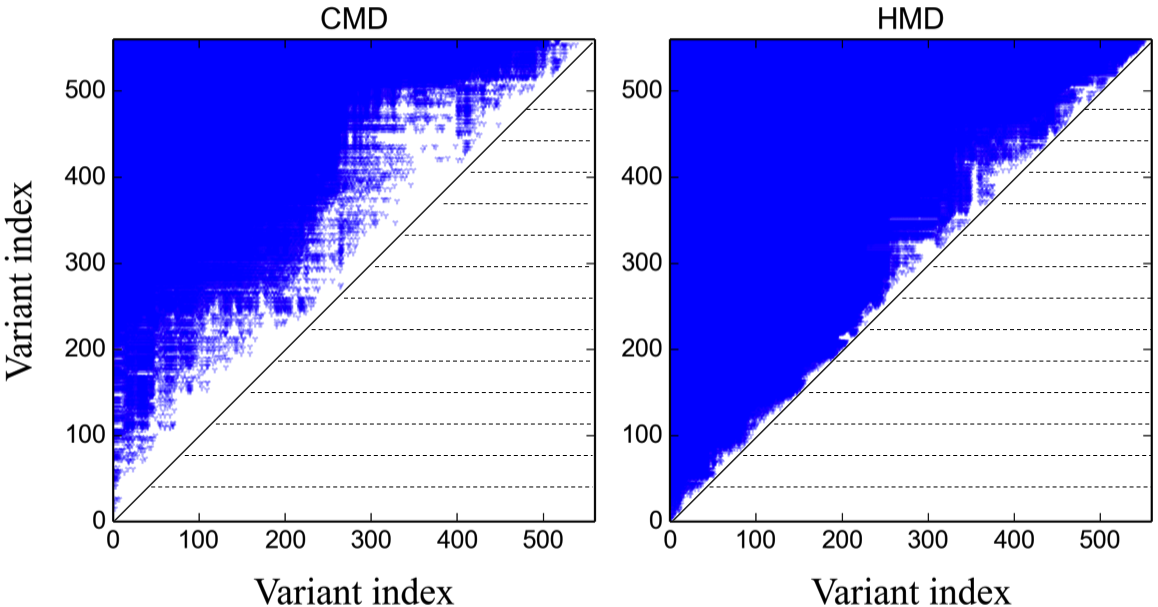
\includegraphics[width=\figSizeEightyFive]{ch06_patterns/figures/StatisticalDiff.png}
	\end{center}
	\caption{Matrix indicating the statistical significance of the performance difference between every variant pair for the \acrshort{msds_iitm_cmd} and the \acrshort{msds_iitb_hmd}. Variant pairs where the difference in the performance is statistically significant are marked by dots.}
	\label{fig:patterns_statistical_significance_similarity_evaluation}
\end{figure}


The MAP scores and the details of parameter settings for the \acrshort{msds_iitb_hmd} dataset are shown in~\tabref{tab:melodic_similarity_results} (bottom half). Compared to the \acrshort{msds_iitm_cmd}, the best MAP score for the \acrshort{msds_iitb_hmd} is higher (0.55). Amongst the top ranked variants there is no consensus on the sampling rate of the melody representation. All the top ranked variants have the same parameter values except the sampling rate. This suggests that the sampling rates considered in this study have no significant effect on the melodic similarity for the \acrshort{msds_iitb_hmd}. This can be attributed to the fact that the recordings in the \acrshort{msds_iitb_hmd} are slow-medium tempo music pieces that do not have fast oscillatory melodic movements, as was the case with the \acrshort{msds_iitm_cmd}.  Furthermore, for the \acrshort{msds_iitb_hmd}, we observe that the variants using $N_{\mathrm{tonic}}$, $N_{\mathrm{tonicQ12}}$ or $N_{\mathrm{tonicQ24}}$ perform better than the ones using $N_{\mathrm{mean}}$, which is in contrast to the observation for the \acrshort{msds_iitm_cmd}. This is primarily because in Carnatic music in our datasets there are many cases where a pattern recurs in a different octave within the same recording, whereas, in Hindustani music, such cases are rare. In general, we see that the \gls{dtw}-based distance performs better than the euclidean distance, and the \gls{dtw} variant without a global constraint ($D_{\mathrm{DTW\_L1\_G90}}$ or $D_{\mathrm{DTW\_L0\_G90}}$) is preferred. This implies that the repeated instances of melodic patterns in IAM (specifically in Hindustani music) have large non linear timing variations.

To assess the statistical significance of the results we compare every possible pair of the variants ($^{560}C_{2}$ = 156520 comparisons). The results are shown in~\figref{fig:patterns_statistical_significance_similarity_evaluation}, where both the axes are the index of the variants in the ranked list. For every variant pair with index $i$ and $j$, we mark the pixel~($i$,$j$) if the difference is statistically significant. From~\figref{fig:patterns_statistical_significance_similarity_evaluation} we see that a majority of variant pairs have a statistically significant difference in the MAP scores. This indicates that the task of computing melodic similarity is sensitive to the choice of parameters and processing steps, and a small change in the choices made in a variant can lead to a significantly different MAP score. Furthermore, as the marked pixels are higher in number for the \acrshort{msds_iitb_hmd}, this sensitivity is even higher for the \acrshort{msds_iitb_hmd} compared to the \acrshort{msds_iitm_cmd}.


\begin{figure}
	\begin{center}
		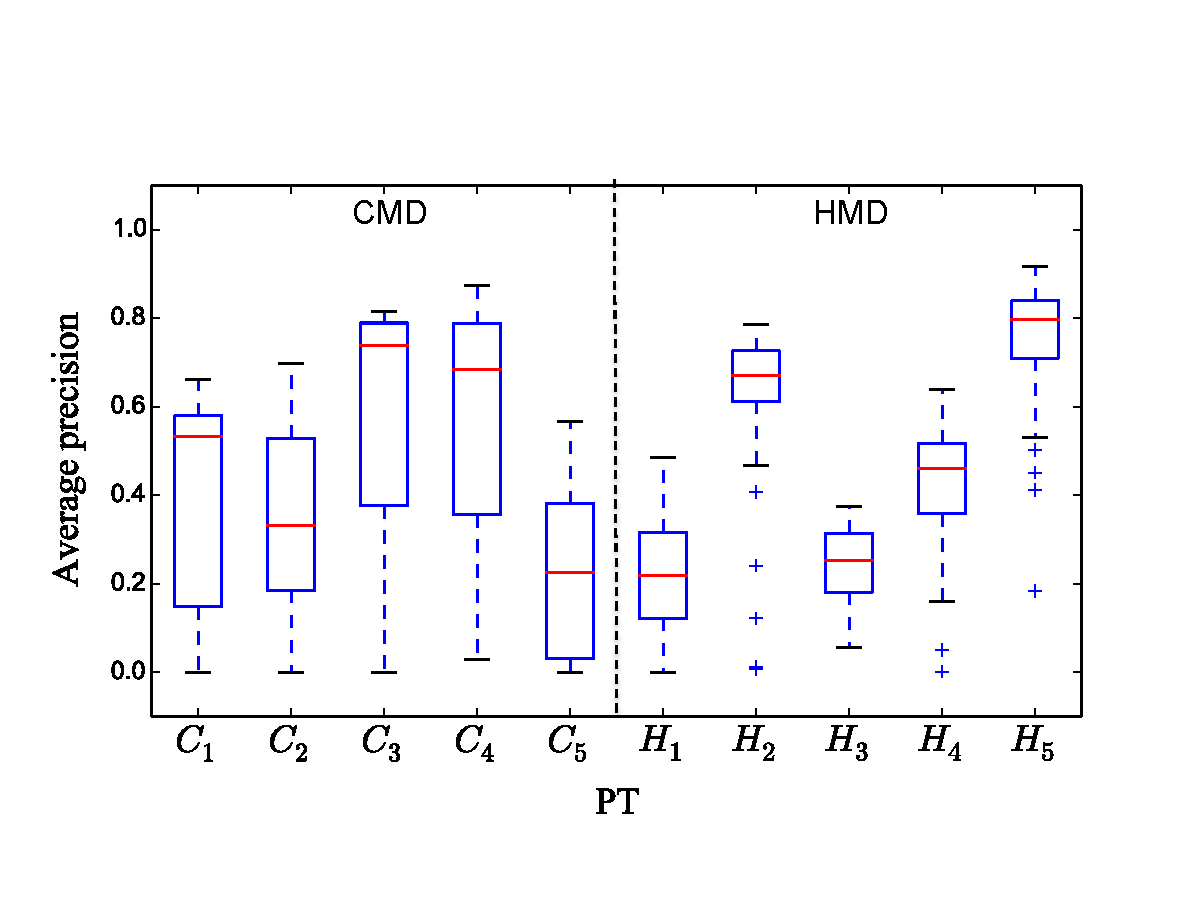
\includegraphics[width=\figSizeEightyFive]{ch06_patterns/figures/CMD_HMD_CW_MAP.pdf}
	\end{center}
	\caption{Boxplot of the average precision values for each pattern type~(PT) in the \acrshort{msds_iitm_cmd} and the \acrshort{msds_iitb_hmd}.}
	\label{fig:patterns_similarity_evaluation_results_boxplot}
\end{figure}


To analyze the consistency in performance across pattern types, we present the boxplot of the average precision values for each pattern type in~\figref{fig:patterns_similarity_evaluation_results_boxplot}. For this, we consider only the top performing variant for each dataset. We see that the MAP scores vary considerably across pattern types for both the \acrshort{msds_iitm_cmd} and the \acrshort{msds_iitb_hmd}. Furthermore, we observe that the intra pattern type variance of the MAP scores is higher for the \acrshort{msds_iitm_cmd} as compared to the \acrshort{msds_iitb_hmd}. In addition, we observe that the pattern types $H_2$ and $H_5$ have a higher MAP value compared to other pattern types in the \acrshort{msds_iitb_hmd}. Interestingly, $H_2$ and $H_5$ are also the pattern types for which $L_{\mathrm{std}}$ is lower and $\#Occ$ is higher than others in the \acrshort{msds_iitb_hmd} (\tabref{tab:categorywise_details_melodic_similarity_dataset}). This correlation is not evident in the \acrshort{msds_iitm_cmd}, since $L_{\mathrm{std}}$ is small for all pattern types. 


\begin{table} 
	\begin{centering}
		\tabcolsep = 0.12cm
		\begin{tabular}{ c | c c c c c}
			\tabletop
			Dataset   	& 	MAP	&	Srate		&	Norm 	&	TScale 		&	Dist \\	
			\tablemid
			\multirow{3}{*}{\acrshort{msds_iitm_cmd}}   	
			& 	0.279 	&	$S_{67}$		&	$N_{\mathrm{mean}}$ 	&	$U_{\mathrm{on}}$		&	$D_{\mathrm{DTW\_L1\_G10}}$\\	
			& 	0.277 	&	$S_{67}$		&	$N_{\mathrm{tonicQ12}}$ 	&	$U_{\mathrm{on}}$		&	$D_{\mathrm{DTW\_L1\_G10}}$\\	
			& 	0.275	&	$S_{100}$		&	$N_{\mathrm{tonicQ12}}$ 	&	$U_{\mathrm{on}}$		&	$D_{\mathrm{DTW\_L1\_G10}}$\\	
\tablemid
			\multirow{3}{*}{\acrshort{msds_iitb_hmd}}   	
			& 	0.259	&	$S_{40}$		&	$N_{\mathrm{tonicQ12}}$ 	&	$U_{\mathrm{on}}$		&	$D_{\mathrm{DTW\_L1\_G90}}$\\	
			& 	0.259 	&	$S_{100}$		&	$N_{\mathrm{tonicQ12}}$ 	&	$U_{\mathrm{on}}$		&	$D_{\mathrm{DTW\_L1\_G90}}$\\	
			& 	0.259 	&	$S_{67}$		&	$N_{\mathrm{tonicQ12}}$ 	&	$U_{\mathrm{on}}$		&	$D_{\mathrm{DTW\_L1\_G90}}$\\	
			\tablebot		
		\end{tabular}
		\caption{MAP score and the details of parameter settings for the three best performing variants for the \acrshort{msds_iitm_cmd} and the \acrshort{msds_iitb_hmd} dataset. These results are corresponding to the experiment where target patterns' length is not read from the ground-truth annotations but is considered to be same as the query pattern length. Srate: sampling rate of the melody representation, Norm: normalization technique, TScale: uniform time-scaling and  Dist: distance measure.}
		\label{tab:melodic_similarity_results_var2}
	\end{table}


So far we have considered segmented melodic patterns obtained using ground-truth annotations. For large audio archives such annotations are rarely available~(\secref{sec:patterns_melodic_pattern_discovery}). To simulate a retrieval scenario where the pattern boundaries are not known \textit{a priori}, we consider a simple extension to the experiment by assuming the target pattern length to be equal to the length of the query pattern. We evaluate all 560 variants of the method as done above on both the datasets under this experimental setup. In~\tabref{tab:melodic_similarity_results_var2} we show the MAP scores of the top performing variants for both the datasets \acrshort{msds_iitm_cmd} and \acrshort{msds_iitb_hmd}. We find that the MAP score for the best performing variant decreases from 0.41 to 0.28 and 0.55 to 0.26 for the \acrshort{msds_iitm_cmd} and the \acrshort{msds_iitb_hmd}, respectively. This indicates that the melodic similarity computation task becomes much more challenging in the absence of an accurate melodic segmentation method. 



It is worth mentioning that compared to the previous studies~\cite{Ishwar2013, Ross2012b} we consider more number of pattern types and evaluate the performance of a variant using all annotated patterns as a query. Hence, the results presented are more comprehensive and reliable.





\section{Improving Melodic Similarity in Indian Art Music}
\label{sec:patterns_improving_melodic_similarity}

\subsection{Partial Transcription}
\label{partial_transcription}

We perform a partial melody transcription to automatically segment and identify the steady svar regions in the melody. Note that even the partial transcription of the melodies is a non-trivial task, since we desire a segmentation that is robust to different melodic ornaments added to a svar where the pitch deviation from the mean svar frequency can be up to 200\,Cents. In Figure~\ref{fig:flatCompressionExample} we show such an example of a steady svar region ($P_{1a}$ from 3-6\,s) where the pitch deviation from the mean svar frequency is high due to added melodic ornaments. Ideally, the melodic region between 1 and 6\,s should be detected as a single svar segment.

We segment the steady svar regions using a method described in~\cite{gulati2014Landmark}, which addresses the aforementioned challenges. A segmented svar region is then assigned a frequency value corresponding to the peak in an aggregated pitch histogram closest to the mean svar frequency. The pitch histogram is constructed for the entire recording and smoothened using a Gaussian window with a variance of 15 cents. As peaks of the normalized pitch histogram, we select all the local maximas where at least one peak-to-valley ratio is greater than 0.01. For a detailed description of this method we refer to~\cite{gulati2014Landmark}. 

%\vSqueezeSmall 
\subsection{Svar Duration Truncation}
\label{svara_duration_trucation}
After segmenting the steady svar regions in the melody we proceed to truncate the duration of these regions. We hypothesize that, beyond a certain value $\delta$, the duration of these steady svar regions do not change the identity of a melodic phrase (i.e.~the phrase category). We experiment with 7 different truncation durations $\delta = \lbrace$ 0.1\,s, 0.3\,s, 0.5\,s, 0.75\,s, 1\,s, 1.5\,s, 2\,s$\rbrace$ and select the one that results in the best performance. In Figure~\ref{fig:flatCompressionExample}
we show an example of the occurrences of a melodic phrase both before ($P_{1a}$, $P_{2a}$) and after ($P_{1b}$, $P_{2b}$) the svar duration truncation using $\delta = 0.1$\,s. This example clearly illustrates that the occurrences of a melodic phrase after duration truncation exhibit lower degree of non-linear timing variations. We denote this method by $M_{DT}$.

\subsection{Complexity Weighting}
\label{sec:complexity_invariance_weighting}

The complexity weighting that we apply here to overcome the shortcoming of the distance measure in distinguishing two time series with different complexities is discussed in~\cite{batista2011complexity}. We apply a complexity weighting ($\alpha$) to the \gls{dtw}-based distance ($D_{DTW}$) in order to compute the final similarity score $D_{f}=\alpha D_{DTW}$. We compute $\alpha$ as:


\begin{equation}
\begin{gathered}
\alpha = \frac{\max(C_i,C_j)}{\min(C_i, C_j)};\hspace{1.5em} C_i = \sqrt[2]{\sum_{i=1}^{N-1} (p_{i}-p_{i+1})^2}\\
\end{gathered}
\label{complexity_estimate_batista}
\end{equation}

\noindent where, $C_i$ is the complexity estimate of a melodic phrase of length $N$ samples and $p_i$ is the pitch value of the $i^{\mathrm{th}}$ sample. We explore two variants of this complexity estimate. One of these variants is already proposed in~\cite{batista2011complexity} and is described in equation~\ref{complexity_estimate_batista}. We denote this method variant by $M_{CW1}$. We propose another variant that utilizes melodic characteristics of Carnatic music. This variant takes the number of saddle points in the melodic phrase as the complexity estimate~\cite{Ishwar2013}. This method variant is denoted by $M_{CW2}$. As saddle points we consider all the local minimas and the local maximas in the pitch contour which have at least one minima to maxima distance of half a semitone. Since such melodic characteristics are predominantly present in Carnatic music, the complexity weighting is not applicable for computing melodic similarity in Hindustani music.


\section{Melodic Pattern Discovery in Sizable Audio Collections}
\label{sec:patterns_melodic_pattern_discovery}

\subsection{Method}


\subsubsection{Pre-processing}
\label{sec:preprocessing}

%\begin{figure}
%	\begin{center}
%		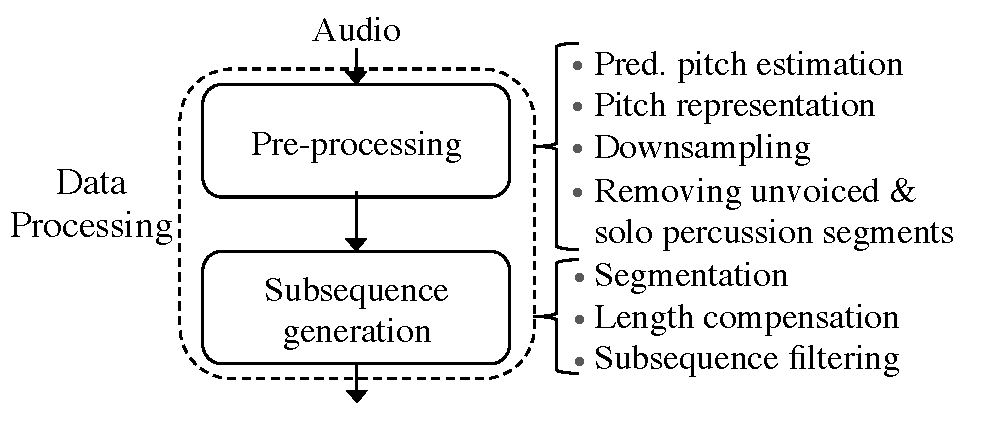
\includegraphics[width=\columnwidth]{figures/blockDiagram_DataProc.pdf}
%	\end{center}
%	\caption{Block diagram of the data processing module.}%\vspace{-1em}
%	\label{fig:blockDiagramDataProc}
%\end{figure}


The steps involved in the pre-processing block are shown in Fig.~\ref{fig:blockDiagramDataProc}. A brief description of each of these steps is given below:

\paragraph{a) Predominant Pitch Estimation} We consider melody as the predominant pitch in the audio signal and estimate it using the method proposed by Salamon and G\'omez~\cite{Salamon2012}. This method performed very favorably in an international MIR evaluation campaign focusing on a variety of music genres, including IAM\footnote{\url{http://nema.lis.illinois.edu/nema_out/mirex2011/results/ame/indian08/summary.html}}. We use the implementation available in Essentia~2.0~\cite{essentia}, an open-source C++ library for audio analysis and content-based MIR. We use a frame size of 46\,ms and a hop size of 4.44\,ms. All other parameters are left to their default values. Before pitch estimation, we apply an equal-loudness filter using the default set of parameters. Noticeably, the predominant pitch estimation algorithm also performs voicing detection, which is used in the later part of our data processing methodology to filter unvoiced segments (Fig.~\ref{fig:blockDiagramDataProc}).%\vspace{0.5em}



\paragraph{b) Pitch Representation} For the pitch representation to be musically relevant, the pitch values are converted from Hertz to Cents (logarithmic scale). For this conversion we additionally consider the tonic pitch of the lead artist as the reference frequency (i.e.,~0\,Cent corresponds to the tonic pitch). Thus, our representation becomes independent of the tonic of the lead artist, which allows a meaningful comparison of melodies of two distinct recordings (even if sung by two different artists in different tonic pitches). The tonic of the lead artist is identified automatically using a classification-based multi-pitch approach~\cite{Gulati2014Tonic}. We use the implementation of this method available in Essentia with the default set of parameters.%\vspace{0.5em}



\paragraph{c) Downsampling} In order to reduce the computational cost, we downsample the predominant pitch sequence (Fig.~\ref{fig:blockDiagramDataProc}). We derive the new sampling rate using the autocorrelation (ACR) of short-time pitch segments generated using a sliding window of 2\,s. We compute the ACR of all possible pitch segments in the entire dataset for different lags $l$, $l\in \lbrace0,1,\dots30\rbrace$, and examine the histogram of normalized ACR values at each lag (Fig.~\ref{fig:ACRHistogram}). %The ACR of a pitch segment is normalized by its value at $l=0$ before computing the histogram. 
We select the lag at which the third quartile Q3 has an ACR value of 0.8, which corresponds to a sampling rate of 22.22\,ms. We informally found that this sampling rate generally preserves melodic nuances and rapid pitch movements while reducing the computational requirements of the task. In the literature, we could not find any reference for this sampling rate of the melody. Thus, our quantitative derivation could be useful for further studies.



\paragraph{d) Solo Percussion Removal} A concert of Carnatic music typically contains a solo percussion section, referred as {\it Tani Avartana} or {\it Tani} in short. Its duration typically varies from 2 to 25\,min. Since the main percussion instrument in Carnatic music, the {\it m\d{r}da\.{n}ga\.{m}}, has tonal characteristics, the pitch estimation algorithm tracks the pitch of the m\d{r}da\.{n}ga\.{m} strokes instead of detecting this section as an unvoiced segment. Hence, we dedicate an extra effort to discard such segments using a classification-based approach (Fig.~\ref{fig:blockDiagramDataProc}). To feed the classifiers we extracted 13~MFCC coefficients, spectral centroid, spectral flatness and pitch salience (c.f.~\cite{slaney1998auditory}) from the audio signal using Essentia. We iterated over 23, 46 and 92\,ms frame sizes and chose the one which resulted in a better classification accuracy. We set the hop size as half the frame size and all other parameters to their default values. Next, we computed means and variances of these features over 2\,s non-overlapping segments. For training, we used a labeled audio music dataset containing 1.5~hours of mixed voice and violin recordings and 1.5~hours of solo percussion recordings. To assess the performance of the extracted features, we performed a leave-one-out cross-validation. We experimented with five different algorithms exploiting diverse classification strategies~\cite{Hastie09BOOK}: decision trees (Tree), $K$~nearest neighbors (KNN), naive Bayes (NB), logistic regression (LR), and support vector machines with a radial basis function kernel (SVM). We used the implementations available in scikit-learn version~0.14.1~\cite{scikitlearn}. We used the default set of parameters with few exceptions to avoid over-fitting and to compensate for the uneven number of instances per class. We set \texttt{min\_} \texttt{samples\_split=10} for Tree, \texttt{fit\_prior=False} for NB, \texttt{n\_neighbors=5} for KNN, and for LR and SVM \texttt{class\_weight=`auto'}. The combination of the frame size of 46\,ms and the SVM classifier yielded the best performance (96\% accuracy), with no statistically significant difference to the performance with the Tree (95.5\%) and the KNN (95\%), for the same frame size. We finally chose KNN because of its low complexity.


%\begin{figure}
%	\begin{center}
%		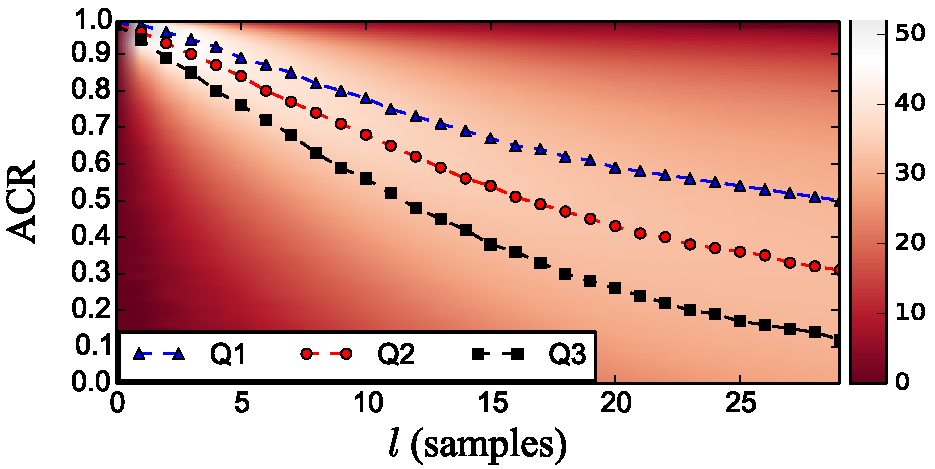
\includegraphics[keepaspectratio = true, height=4cm, scale=1]{figures/ACRHistogram.pdf}
%	\end{center}
%	\caption{Histograms of ACR values (histogram value is indicated by the colormap on the right; for ease of visualization, we compress the range of the histogram values by taking its fourth root). Q1, Q2 and Q3 denote the three quartile boundaries of the histogram. }
%	\label{fig:ACRHistogram}
%\end{figure}

\subsubsection{Subsequence Generation}
\label{sec:subsequencegeneration}
The steps involved in generating candidate subsequences are as follows:
\paragraph{a) Segmentation} Due to the lack of reliable methods for segmentation of melodic patterns in IAM~\cite{gulati2014Landmark}, we generate pitch subsequences by using a sliding window of length $W_l$ with a hop size of one sample (22\,ms). Given no quantitative studies investigating the length of the melodic patterns in Carnatic music, we make a choice of $W_l = 2$\,s based on recommendations from a few Carnatic musicians. Since unvoiced segments are removed from the pitch sequence at the pre-processing step, a window can include pitch samples separated by more than $W_l$ seconds. To handle these cases, we use the time stamps of the first sample ($T_1$) and the last sample ($T_2$) in a window. We filter out all subsequences for which $T_2-T_1 > W_l + \Phi$. We select $\Phi =0.5$\,s to account for the short pauses during a phrase rendition. This value was empirically set to differentiate between inter- and intra-phrase pauses.%\vspace{0.5em}


\paragraph{b) Subsequence Filtering} A subsequence may contain a segment of the pitch contour corresponding to a single musical note, where the pitch values are nearly constant. Such musically uninteresting patterns are discarded in a filtering stage (Fig.~\ref{fig:blockDiagramDataProc}). The criterion for discarding such subsequences is summarized below:
%\begin{equation}
%\begin{aligned}
%f_i& = 
%\begin{cases}
%    1, & \text{if } S_i\geq T_{\text{std}}\\
%    0, & \text{otherwise}
%\end{cases}\hspace{0.6cm}|\hspace{0.6cm}
%\beta&=\sum_{i=0}^{W_n}f_i
%\end{aligned}
%\label{eq:subsequencefiltering}
%\end{equation}%\vspace{-1em}
\begin{equation*}
\beta =\sum_{i=0}^{W_n} \Theta\left(S_i\geq T_{\text{std}}\right),
\end{equation*}


\noindent where $\beta$ is the flatness measure of a subsequence, $W_n$ denotes its number of samples, $\Theta(z)$ is a Heaviside step function yielding $\Theta(\text{true})\!=\!1$ and $\Theta(\text{false})\!=\!0$, and $S_i$ is the standard deviation at the $i$-th sample of a subsequence, computed using a window of length $W_{\text{std}}$ centered at sample $i$. %The threshold $T_{\text{std}}$ determines if a sample belongs to a flat region or not.
In order to determine the optimal values of $W_{\text{std}}$ and $T_{\text{std}}$, we manually labeled a number of regions in pitch contour as `flat' and `non-flat' for 4 excerpts in our database. We iterated over different parameter values and analyzed the resultant ROC curve (Fig.~\ref{fig:ROC}). %In  we show the ROC curve obtained for $W_{\text{std}} \in \lbrace100,200,400\rbrace$\,ms. 
Doing so, we found that $W_{\text{std}}=200$\,ms resulted in the best performance and that the knee of the curve corresponded to $T_{\text{std}}=45$\,Cents. Having a value of $\beta$ for each subsequence, we finally filter out the ones for which $\beta \leq \gamma W_n$, using $\gamma = 0.8$. The latter was set by visual inspection.

%\begin{figure}
%	\begin{center}
%		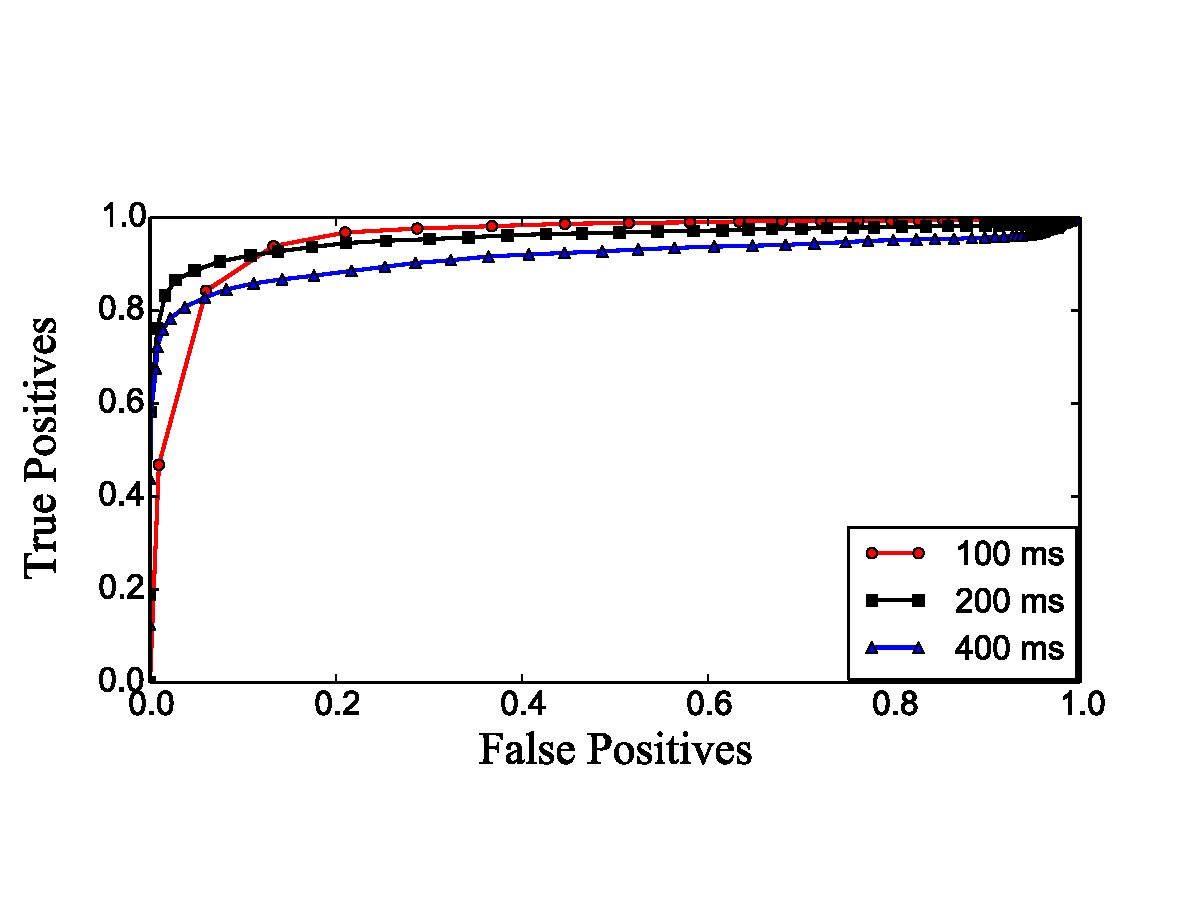
\includegraphics[keepaspectratio = true, height=4cm, scale=1]{figures/ROCFlatness.pdf}
%	\end{center}
%	\caption{ROC curves for `flat' and `non-flat' region classification for different values of window length ($W_{\text{std}}$) used for selecting an optimal value of standard deviation $S_i$.}
%	\label{fig:ROC}
%\end{figure}


After the data processing step, we retain around 17.5 million pattern candidates for our entire dataset. If no subsequence filtering is applied, a sampling rate of 225\,Hz for pitch sequence amounts to nearly 300~million pattern candidates for a database as big as ours.

\subsection{Intra-recording Pattern Discovery}
\label{sec:intraRecordingPatternDiscovery}

We perform an exact pattern discovery by computing the similarity between every possible subsequence pair obtained within an audio recording. We regard the top $N=25$ closest subsequence pairs in each recording as seed patterns. We omit overlapping subsequences in order to avoid trivial matches and additionally constrain the top $N$ seed pattern pairs to be mutually non-overlapping. Due to this constraint for some recordings we obtain less than 25 pattern pairs. In total, for all the recordings, nearly 1.4 trillion \gls{dtw} distance computations are done to obtain 79,172 seed patterns.

\subsubsection{Melodic Similarity}
\label{MelodicSimilarity}
We compute melodic similarity between two subsequences using a \gls{dtw}-based distance measure~\cite{Sakoe78TASLP}. We use a step condition of $\lbrace(1,0), (1,1), (0,1)\rbrace$ and the squared Euclidean distance as the cost function. We do not use any penalty for insertion and deletion. These choices are made in order to allow lower bounding (see below). In addition, we apply the Sakoe-Chiba global constraint with the band width set to 10\% of the pattern length. This constraint may be sufficiently large for accounting time warpings in melodic repetitions in Carnatic music.

\subsubsection{Lower Bounding \gls{dtw}}
\label{LowerBoundingDTW}
To make \gls{dtw} distance computations tractable for such a large number of subsequences we apply cascaded lower bounds~\cite{Rakthanmanon2013}. In particular, we use FL (first-last) lower bound and LB\_Keogh bound for both query to reference and reference to query matching. Besides, we apply early abandoning, both during the computation of lower bounds as well as during the \gls{dtw} distance computation~\cite{Rakthanmanon2013}. 

\subsubsection{Pattern Length Compensation}
\label{PatternLengthCompensation}
Along with the local non-linear time warpings, the overall length of a melodic pattern may also vary across repetitions. For example, a melodic pattern of length 2\,s might be sung in 2.2\,s in a different position in the song. We handle this by using multiple time scaled versions of a subsequence in the distance computation. This technique is also referred to as local \gls{dtw} and is shown to have tighter lower bounds~\cite{Zhu2003}. It should be noted that typically such issues are addressed by using a subsequence variant of the \gls{dtw} distance measure. However, the lower bounding techniques we used during the \gls{dtw} distance computation do not work for the subsequence variant of the \gls{dtw}. 

For every subsequence, we generate five subsequences by uniformly time scaling it by a factor of $\alpha \in I_{\text{intp}} =\lbrace 0.9, 0.95, 1, 1.05, 1.1\rbrace$, such that the length of the resulting subsequences is $W_l$. We use cubic interpolation for uniformly time scaling a subsequence. Since these 5 interpolation factors increase the computational cost by a factor of 25, we assume that the distance between a subsequence pair $X_{1.0}$ and $Y_{1.05}$ is very close to the distance between the pair $X_{1.05}$ and $Y_{1.1}$ (the sub-index denotes the interpolation factor $\alpha$). Following this rationale, we can avoid the distance computation between 16 of the 25 combinations without a significant compromise on accuracy.

\subsection{Inter-recording Pattern Detection}
\label{sec:patternSearch}


We consider every seed pattern as a query (79,172 in number) and perform an exhaustive search over all the subsequences obtained from the entire audio music collection (nearly 17.5 million in number). For every seed pattern we store top $M=200$ closest matches (referred to as search patterns). Here also for every subsequence we consider 5 uniformly  scaled subsequences in the distance computation. For inter-recording pattern detection also use the same similarity measure and lower bounding techniques as used in intra-recording pattern discovery block (Sec.~\ref{sec:intraRecordingPatternDiscovery}). In total, nearly 12.4 trillion \gls{dtw} distance computations are done in this step.



\subsection{Rank Refinement}
\label{sec:rankRefinement}

The lower bounds we use for speeding up distance computations are not valid for any variant of \gls{dtw}. However, once the top matches are found, nothing prevents us from reordering the ranked list using any variant of \gls{dtw}, as we do not need to apply lower bounds in this reduced search space. In this step, we select a \gls{dtw} step condition of $\lbrace(1,2), (1,1), (2,1)\rbrace$ to avoid some pathological warpings of the path. Furthermore, we investigate four different distance measures $d_i$, $i=1,\dots 4$, used in the computation of the \gls{dtw} cost matrix as described below. %(Fig.~\ref{fig:Distances}).
%We choose $d_1 = \delta^2$, $d_2=\delta$, $d_3 = \delta-25$ if $\delta>25$ or %$d_3=0$ otherwise, $d_4 = (\delta-\phi)^{1.5} + \varphi$ if $\delta>100$ or $d_4 %= d_3$ otherwise. 

\begin{equation}
\begin{aligned}
d_1& = \delta \hspace{.5em};&
d_3& = 
\begin{cases}
\delta-25, & \hspace{1cm} \text{if } \delta >25\\
0, & \hspace{1cm}\text{otherwise } 
\end{cases}
\\
d_2& = \delta^2 \hspace{.5em};&
d_4 &= 
\begin{cases}
(\delta-\phi)^{1.5} + \varphi, & \text{if } \delta >100\\
d_3, & \text{otherwise}
\end{cases}
\end{aligned}
\label{eq:distances}
\end{equation}



\noindent where $\delta = |p_1-p_2|$ is the city block distance between two pitch values and all numeric values are in Cents. We set $\phi =99.555$ and $\varphi = 74.70$ to maintain point and slope continuity. The formulation for the different $d_i$ is inspired by our own experience and some of the approaches we find in the literature~\cite{Ishwar2013,Rao2014}. We denote the four variants of the rank refinement method by $V_i$, $i=1\dots 4$.

\subsection{Evaluation}


One of the challenges in any data-driven task is evaluation. We here perform a quantitative evaluation based on expert feedback. For the entire dataset we obtain over 15\,million search patterns for each of the rank refinement methods. We divide seed patterns into three categories based on the distance between the seed pairs, which we denote by $D$. Then, to have an equal representation from the range of values of $D$, 200 seed pairs equally distributed among these categories are randomly selected for evaluation (Fig.~\ref{fig:SeedDistanceDistribution}). Seed category boundaries are $\mu \pm 1.5\sigma$, where $\mu$ and $\sigma$ are the mean and the standard deviation of the distribution of $D$. For every selected seed pattern we consider the first 10 search patterns for each of the four rank refinement methods. Thus, in total, we obtain 200 seed pairs and 8,000 search patterns for expert evaluation.

Expert evaluation is performed by a professional Carnatic musician who has received over 20 years of music education. For examining similarity between two melodic patterns, the musician listened to the audio fragments corresponding to these patterns and scored a 0 for melodically dissimilar and a 1 for melodically similar. The musician annotated melodic similarity for each seed pair and between the seed and its search patterns for every rank refinement method.

%\begin{figure}
%	\begin{center}
%		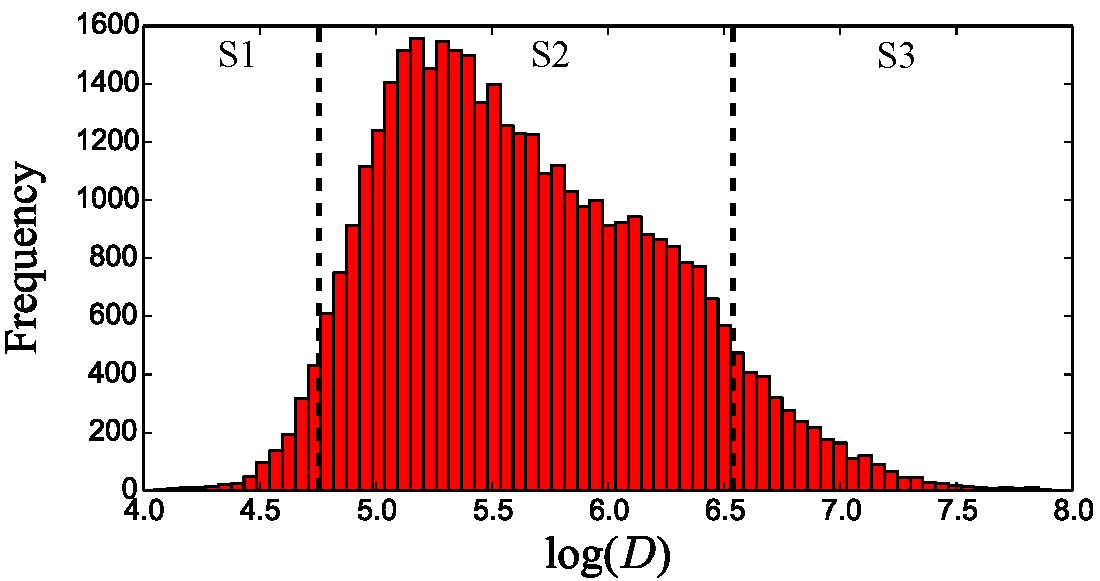
\includegraphics[keepaspectratio = true, height=4cm, scale=1]{figures/SeedDistribution.pdf}\vspace{-1em}
%	\end{center}
%	\caption{Distance distribution of seed patterns. Three seed pattern categories are marked by S1, S2 and S3.}
%	\label{fig:SeedDistanceDistribution}
%\end{figure}

To quantify the musician's assessment of the similarity between the melodic patterns  we use mean average precision (MAP), a typical evaluation measure in information retrieval~\cite{manning2008introduction}, which is also very common in MIR. This way, we have a single number to evaluate the performance of the four different rank refinement methods. For the computation of the MAP scores we consider the total number of relevant patterns as the number of relevant patterns retrieved in the top 10 search results.  For assessing statistical significance we use the Mann-Whitney U test~\cite{mann1947test} with $p < 0.05$. To compensate for multiple comparisons, we apply the Holm-Bonferroni method~\cite{holm1979simple}. Thus, eventually we use a much more stringent criteria than $p < 0.05$ for measuring statistical significance. We use ROC curves to analyze the separation between the distance distribution of melodically similar and dissimilar subsequences~\cite{manning2008introduction}. 

\subsection{Results}


%\begin{figure}
%	\begin{center}
%		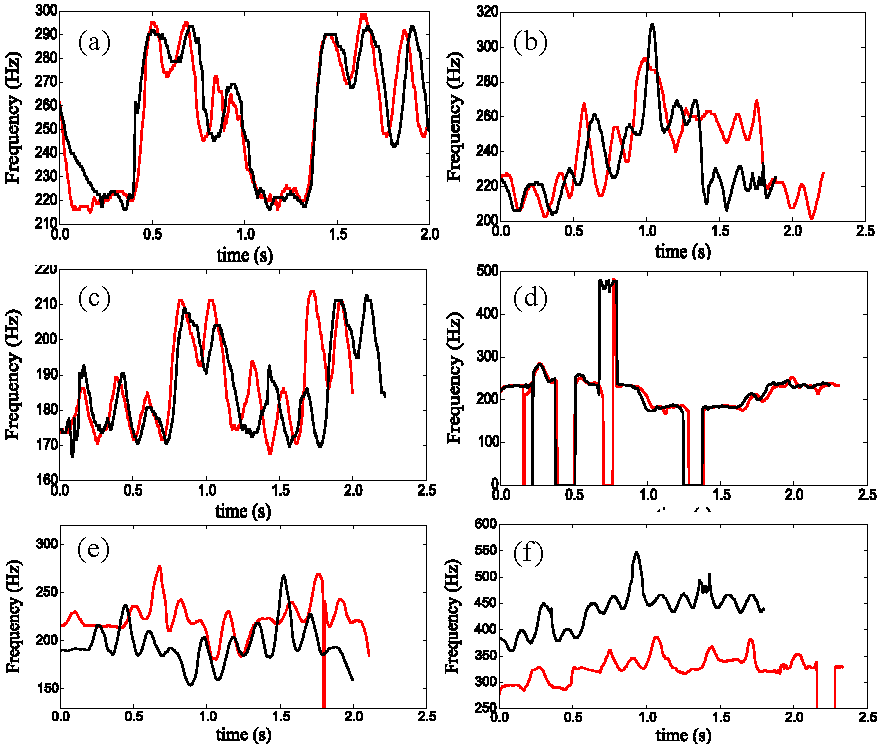
\includegraphics[keepaspectratio = true, width=\columnwidth, scale=1]{figures/PatternPlots/combinedPatterns.pdf}
%	\end{center}
%	\caption{Examples of the discovered melodic patterns. \XXX{S}{J}{I have to put a,b,c,d in the image (later this day)}}%\vspace{-1em}
%	\label{fig:combinedPatterns}
%\end{figure}

Before presenting formal evaluations, we show a few examples of the discovered melodic patterns in Fig.~\ref{fig:combinedPatterns}. Our approach robustly extracts patterns in different scenarios such as large local time warpings~(b), uniform scaling~(c), patterns with silence regions~(d) and across different tonic pitches~(e and f). It is worth mentioning that, during the process of annotation, the musician found several musically interesting results. For example, striking similarity between phrases of two different r\={a}gas, between phrases in sung melodies and the melodies played on instruments (Violin or V\={i}\d{n}a), and phrases sung by different artists. Many of the discovered patterns are the characteristic melodic phrases of the r\={a}ga, which are the primary cues for r\={a}ga recognition. Overall, the  obtained results are musically relevant and can be used to establish meaningful relationships between audio recordings.

It is also interesting to analyze the contribution of different lower bounds in pruning the search space. In Table \ref{tab:computationalStats} we show in percentage the number of times the program counter exits after a lower bound computation with respect to the total number of distance computations. As mentioned before, the total number of distance computations are 1.413 trillion for intra-recording pattern discovery and 12.418 trillion for inter-recording pattern detection. From Table \ref{tab:computationalStats} it becomes evident that the lower bounding methods are more effective in inter-recording pattern detection. This is expected as different songs may correspond to different r\={a}gas and hence use different set of musical notes.


We now proceed to formal evaluations. We first evaluate the performance of the intra-recording pattern discovery task. We find that the fraction of melodically similar seed pairs within each seed category S1, S2 and S3 consistently decreases: 0.98, 0.67 and 0.31, respectively. To further examine the separation between melodically similar and dissimilar seed pairs, we compute the ROC curve (Fig.~\ref{fig:combinedROC}, solid blue line). The knee of such curve corresponds to a precision of approximately 80\% for 10\% of false positive cases. This indicates that the chosen \gls{dtw}-based distance measure is a sufficiently good candidate for computing melodic similarity for the case of intra-recording seed pattern discovery. 

\begin{table} 
	\centering
	\caption{Percentage of exits after a lower bound computation with respect to the total number of distance computations.}
	\label{tab:computationalStats}
	
	\begin{tabular}{ c | c c }
		
		\hline\hline
		Lower bound   	& Intra-rec.(\%)		&	Inter-rec.(\%) \\	
		
		\hline 
		%LB\_KIM\_FL   		& 1.0	&	1.0 \\	
		LB\_KIM\_FL   	& 52	&	45 \\	
		LB\_Keogh\_EQ   	& 23	&	51 \\
		LB\_Keogh\_EC   		& 1	&	3 \\
		%DTW 	& 24	&	1 \\
		\hline\hline
		
	\end{tabular}
	
\end{table}



%\begin{figure}
%	\begin{center}
%		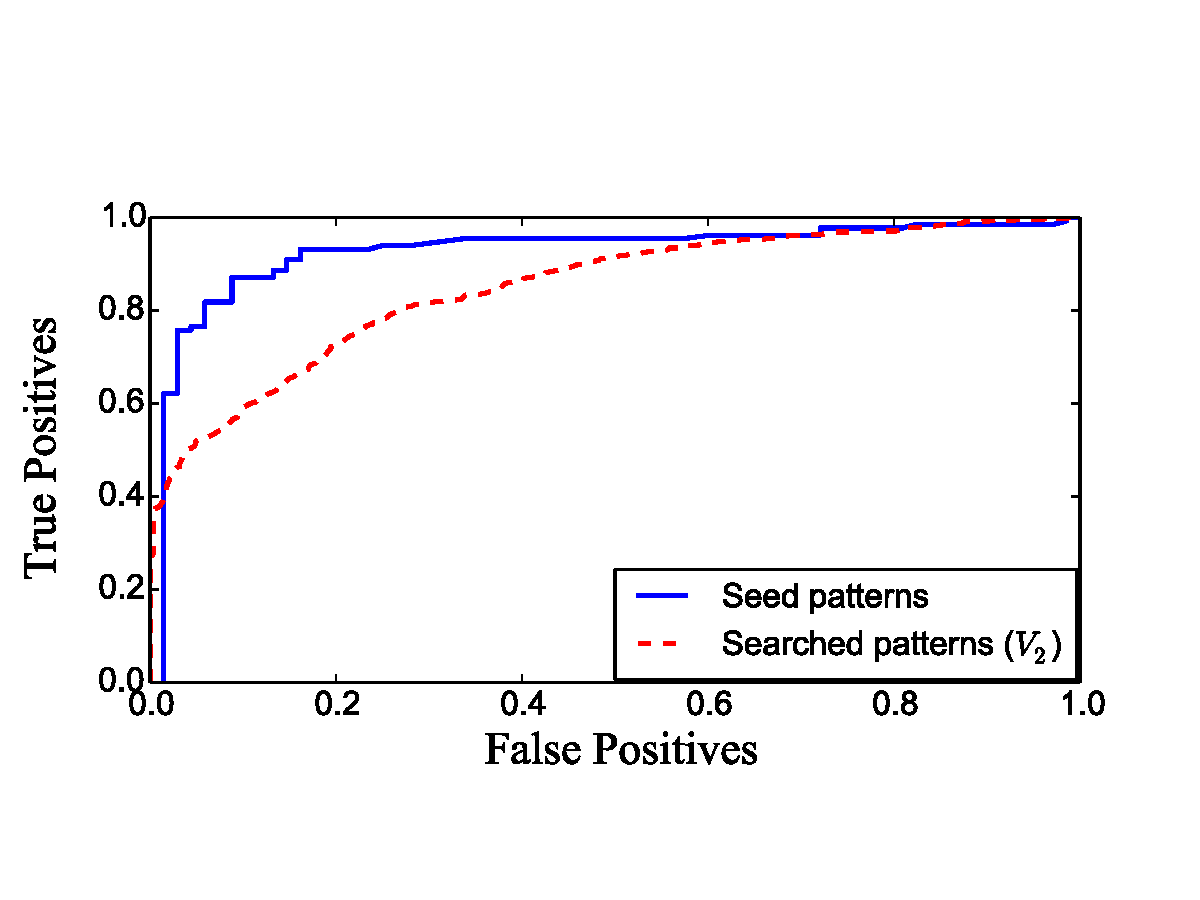
\includegraphics[keepaspectratio = true, height=4cm, scale=1]{figures/seedROC.pdf}
%	\end{center}
%	\caption{ROC curve for seed pairs and search patterns (using $V_2$) in the evaluation set.}%\vspace{-1em}
%	\label{fig:combinedROC}
%\end{figure}

Next, we evaluate the performance of inter-recording pattern detection task and assess the effect of the four \gls{dtw} cost variants of Sec~\ref{sec:rankRefinement} (denoted by $V_1 \dots V_4$). To investigate the dependence of  the performance on the category of the seed pair, we perform the evaluation within each seed category (Table~\ref{tab:meanAveragePrecision}). In addition, we also present a box plot of corresponding average precision values (Fig.~\ref{fig:boxPlotMAP}). In general, we observe that every method performs well for category S1, with a MAP score around 0.9 and no statistically significant difference between each other. For category S2, $V_2$ and $V_3$ perform better than the rest and the difference is found to be statistically significant. The performance is poor for the third category S3 for every variant. The difference in performance between any two methods across seed categories is statistically significant. We observe that MAP scores across different seed categories correlate well with the fraction of melodically similar seed pairs in that category (discussed above). This suggests that patterns which find good matches within a recording (i.e.,~low distance $D$) also correlate with more repetitions across recordings.

Finally, we analyze the distance distribution of search patterns for the best performing method $V_2$ (Fig.~\ref{fig:combinedROC}, dashed red line). We observe that the separability between melodically similar and dissimilar subsequences in this case is poorer than the one obtained for the seed pairs (solid blue line). This indicates that it is much harder to differentiate melodically similar from dissimilar patterns when the search is performed across recordings. This can be attributed to the fact that phrases of two allied r\={a}gas are differentiated based on subtle melodic nuances~\cite{Viswanathan2004}. Hence, one faces a much more difficult task. 

\begin{table} 
	\centering
	\caption{MAP scores for four variants of rank refinement method ($V_i$) for each seed category (S1, S2 and S3).}
	\label{tab:meanAveragePrecision}
	
	\begin{tabular}{ c | c c c c}
		\hline\hline
		Seed Category   & $V_1$		&	$V_2$ & $V_3$	 &	$V_4$ 	\\	
		\hline
		S1 & 0.92    &	0.92		&	0.91    &	0.89\\
		S2 & 0.68    &	0.73		&	0.73    &	0.66\\
		S3 & 0.35    &	0.34    &	0.35    &	0.35\\
		\hline\hline
	\end{tabular}
	
\end{table}

%
%\begin{figure}
%	\begin{center}
%		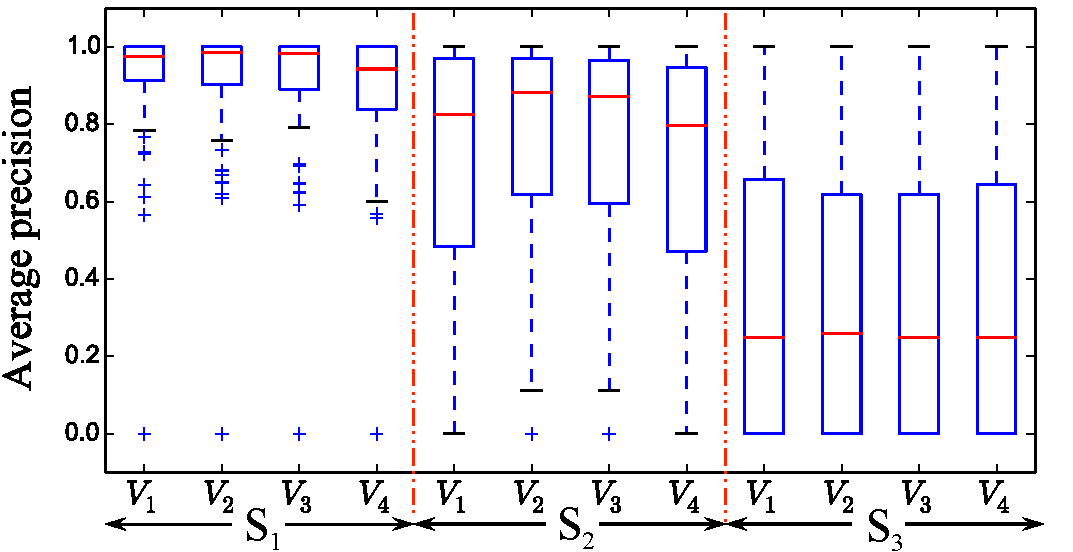
\includegraphics[keepaspectratio = true, width=\columnwidth, scale=1]{figures/boxPlot.pdf}
%	\end{center}
%	\caption{Boxplot of average precision for variants of rank refinement method ($V_i$) for each seed category. }%\vspace{-1em}
%	\label{fig:boxPlotMAP}
%\end{figure}


\section{Characterization of Melodic Patterns}
\label{sec:patterns_characterization_of_melodic_patterns}


\subsection{Method}

\subsection{Melodic Pattern Characterization}
\label{pattern_characterization}

As explained, a discovered melodic pattern can correspond to either a r\={a}ga motif, a composition-specific motif or to a gamaka motif (Section~\ref{sec:introduction}). The aim of the pattern characterization block is to cluster these discovered patterns and to characterize the obtained clusters in order to identify the ones that represent different r\={a}ga motifs. For this, we propose to perform a network analysis as described below.

\subsubsection{Pattern Network Generation}
\label{sec:network_generation}

We start by building an undirected weighted network using the discovered patterns from the previous step. The patterns are considered as the nodes of the network and the edge between any two patterns ($i$, $j$) is weighted based on the distance $D_{ij}$ between the patterns. Noticeably, $D_{ij}$ is computed using the same distance measure as used in the pattern discovery block of Section~\ref{pattern_discovery}. The weight of the edge $W_{ij}$ between the nodes $i$ and $j$ is given by $W_{ij} = e^{\nicefrac{-D_{ij}}{\bar{D}}}$, where, $\bar{D}$ is the mean of $D_{ij}$ over every combination of $i$ and $j$.
%\begin{equation}
%W_{ij} = e^{\nicefrac{-D_{ij}}{\bar{D}}},
%\label{eq:edge_weight}
%\end{equation}
%\noindent where, $\bar{D}$ is the mean of $D_{ij}$ over every combination of $i$ and $j$. 
%We only connect two nodes ($i$, $j$) if the distance between them $D_{ij}$ is less than a threshold $T_B$. Note that $T_B$ is a very lenient threshold and is applied to avoid edges between highly dissimilar melodic patterns so as to reduce the computational complexity during the network analysis. A musically meaningful melodic similarity threshold is derived in the subsequent section. Given $D_{ij} < T_B$.

%It has to be noted that, before generating the network, we remove overlapping melodic patterns. We do this by selecting the pattern among the overlapping patterns that has the lowest distance with the first nearest neighbor. %The resulting network consists of XXX number of nodes and XXX number of edges for the music collection that we consider in this study.

%\begin{figure}
% \begin{center}
% 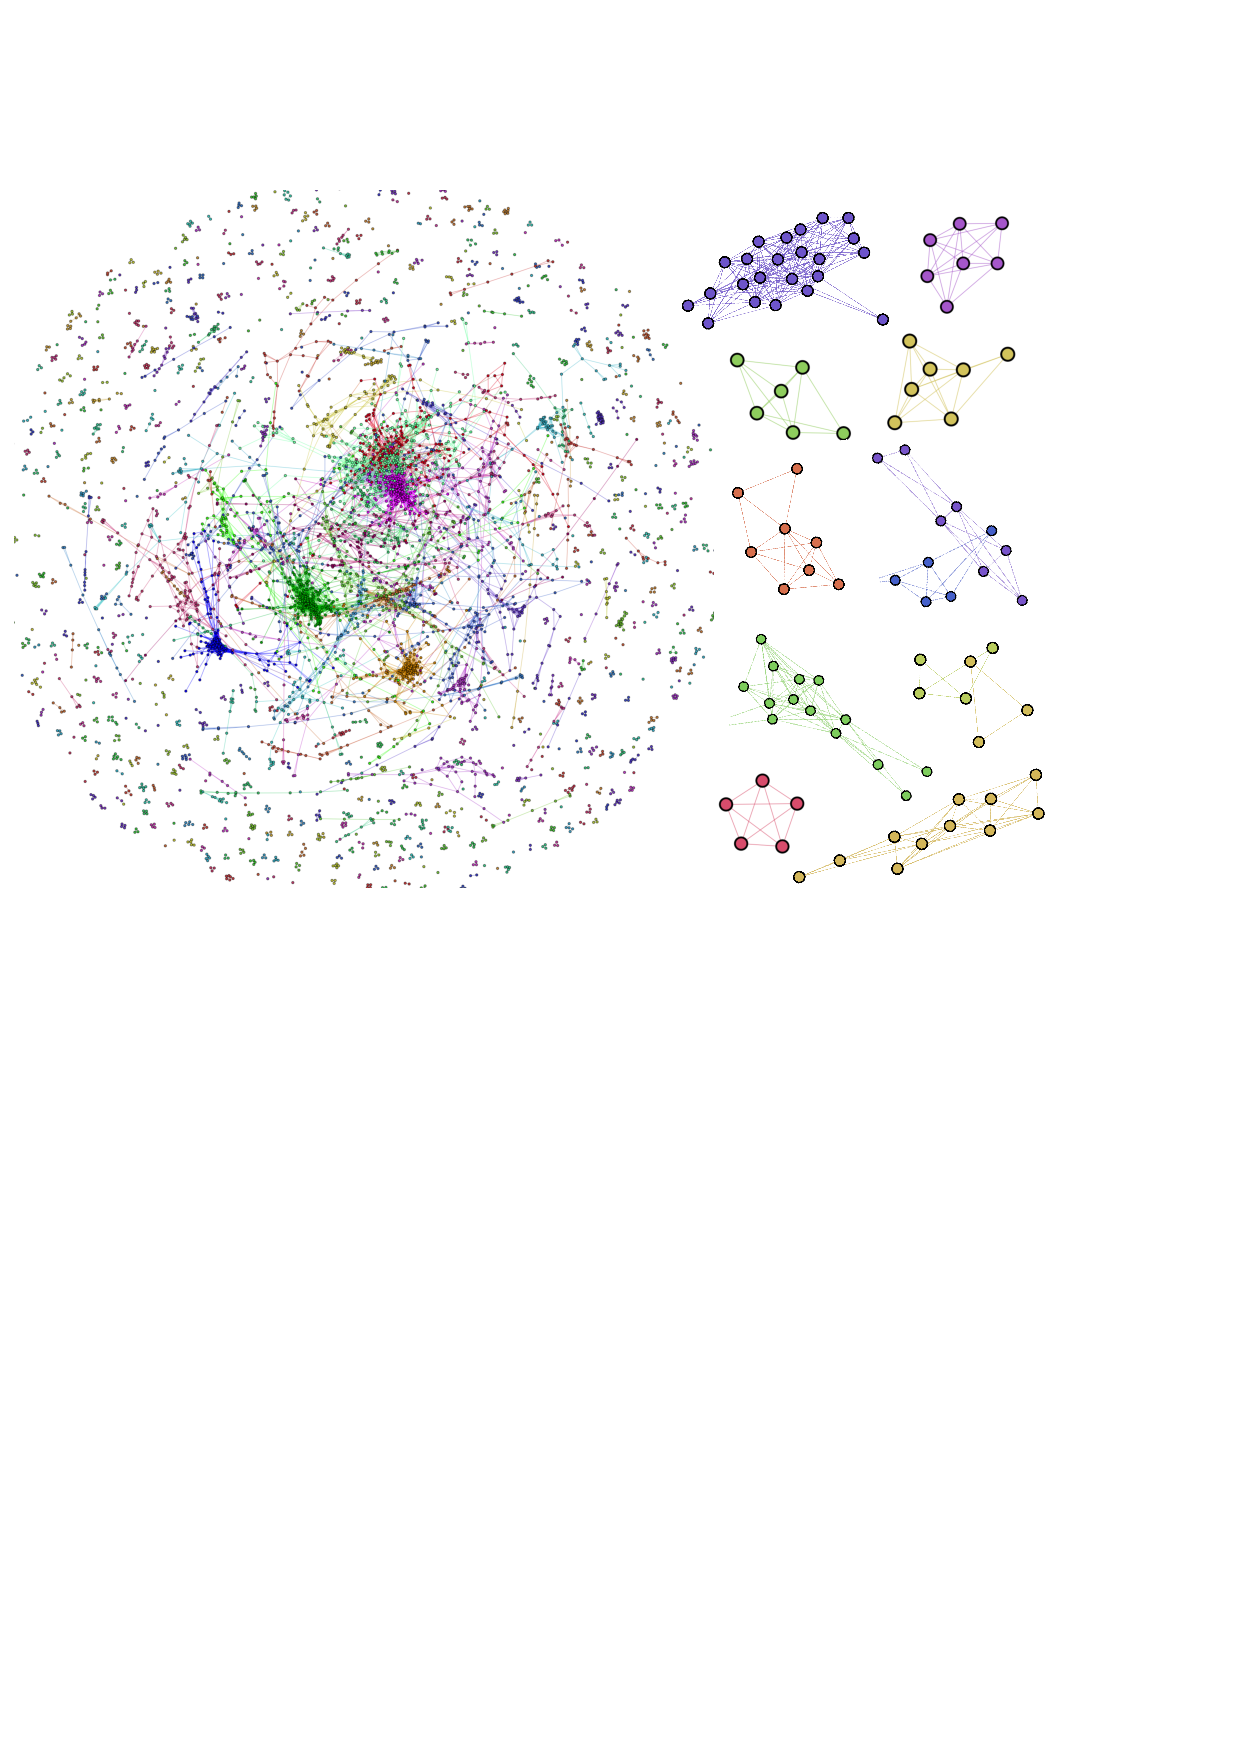
\includegraphics[width=\columnwidth]{figures/networkImages/macOutput/networkWithClusters.pdf}\vSqueezeBig
% \end{center}
% \caption{Graphical representation of the melodic pattern network after filtering by threshold $T_S$. The detected communities in the network are indicated by different colors. Few examples of these communities are shown on the right.}\vSqueezeNormal
% \label{fig:network_and_communities}
%\end{figure}

\subsubsection{Network Filtering}
\label{sec:network_filtering}

The main objective of this processing block is to filter the network to retain only the musically meaningful connections between the nodes. Since the edge weights between the pairs of melodically similar and dissimilar nodes may vary by orders of magnitude, we first consider to exploit this heterogeneity to extract the network's backbone. We therefore need to apply disparity filtering~\cite{Serrano09PNAS} to preserve only the edges that represent statistically significant deviations with respect to a null model of edge weight assignment for every node. The only parameter used in the disparity filtering is the statistical confidence value. We iterate over 5 different confidence values $\lbrace$99.99, 99, 90, 80, 50$\rbrace$. However, as we will show, the application of disparity filtering is found to be quite irrelevant for the present case.

%\begin{figure}
%	\begin{center}
%		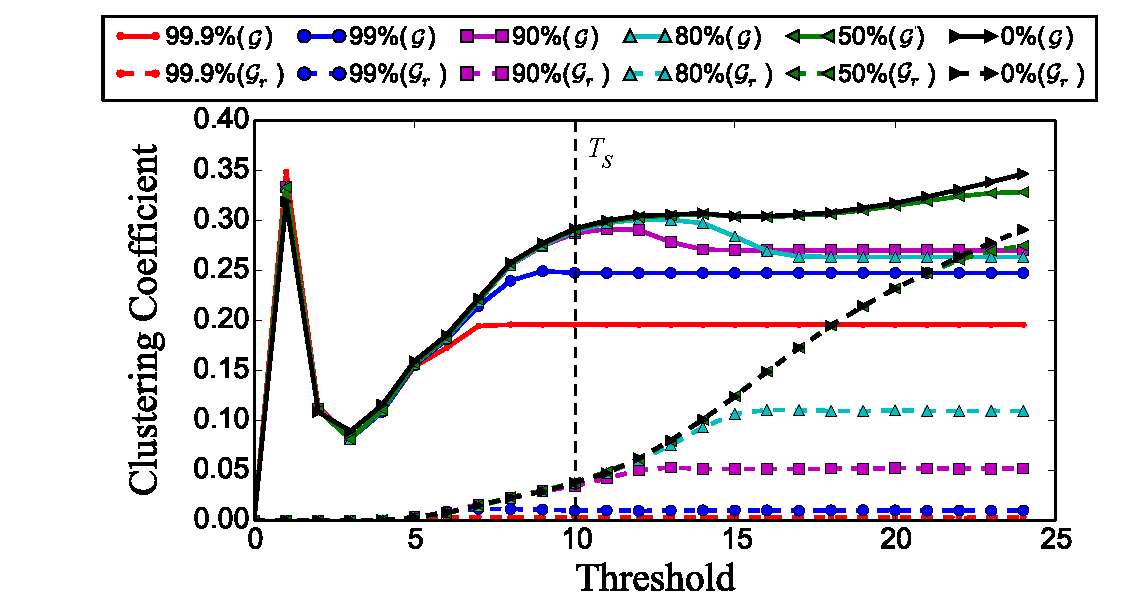
\includegraphics[width=.9\columnwidth]{figures/CC_Curves_shrunk.pdf}\vSqueezeBig
%	\end{center}
%	\caption{Evolution of the clustering coefficient of $\mathcal{G}$ and $\mathcal{G}_r$ over different thresholds and for different statistical confidence values used for disparity filtering (legend).}\vSqueezeNormal
%	\label{fig:cc_curve}
%\end{figure}


We next proceed to filter edges in the network based on a melodic similarity threshold $T_S$. We propose to estimate $T_S$ based on the topological properties of the network. For this, we analyze the evolution of the clustering coefficient of both the obtained network $\mathcal{G}$ and the corresponding randomized network $\mathcal{G}_r$ over a range of similarity thresholds. Clustering coefficient measures the extent to which the nodes in a network tend to cluster together~\cite{newman2003structure}. The randomized network $\mathcal{G}_r$ is obtained by swapping the edges between randomly selected node pairs such that the degree of each node is preserved~\cite{maslov2002specificity}. This way, $\mathcal{G}_r$ can be considered as the maximally random network with that particular degree distribution. In Figure~\ref{fig:cc_curve}, we show the evolution of the clustering coefficient of $\mathcal{G}$ and $\mathcal{G}_r$ over different similarity thresholds (indicated by exponentially spaced bins). In addition, we can also see the clustering coefficient curves for different statistical confidence values used for disparity filtering. The evolution of the clustering coefficients is used for obtaining a similarity threshold as explained below.

We hypothesize that the more musically meaningful $T_S$ is, the higher is the difference between the clustering coefficients of $\mathcal{G}$ and $\mathcal{G}_r$. We therefore select $T_S=10$. Note that even though the similarity threshold corresponding to $T_S=1$ results in a higher value of the clustering coefficient, we reject it because the filtered network consists only of a small number of nodes. These nodes correspond to near-exact pattern repetitions discovered within the same recording~\cite{gulati_SITIS_2014}. Such patterns typically represent composition-specific motifs, and hence are irrelevant in our context. In Figure~\ref{fig:cc_curve}, we also observe that the disparity filtering using a confidence value higher than 80\% significantly lowers the clustering coefficient, which can be attributed to the removal of musically meaningful edges in the network. On the other hand, given $T_S=10$, the disparity filtering with a confidence value lower than 80\% does not significantly affect the clustering coefficient. We can thus conclude that, in the given scenario, disparity filtering does not bring in any clear advantage. Finally, after applying $T_S$, we transform $\mathcal{G}$ to an unweighted network. 


\subsubsection{Community Detection and Characterization}
\label{sec:community_detection}

We next take the unweighted undirected network that results from the previous step, and perform a non-overlapping community detection using the method proposed in~\cite{blondel2008fast}. This method is based on modularity optimization and is parameter-free from the point of view of the user. It has been extensively used in various applications~\cite{fortunato2010community} and can deal with very large networks~\cite{blondel2008fast}. We use the implementation available in networkX~\cite{hagberg-2008-exploring}, a Python language package for exploration and analysis of networks and network algorithms. Using this method for our entire dataset, we obtain around 1800 communities of melodic patterns. 
%For a better understanding of the network obtained after filtering and the detected communities, we show a graphical representation of the network in Figure~\ref{fig:network_and_communities}. We find that many communities comprising large number of nodes in the network correspond to the melodic pattern (Kampita), which occur in several r\={a}gas across compositions and hence have large number of occurrences. We also find that the communities with a relatively smaller number of nodes, which in Figure~\ref{fig:network_and_communities} appear as isolated communities around the periphery often correspond to the r\={a}ga motifs. A few examples of such communities are shown in Figure~\ref{fig:network_and_communities} on the right.

A community $C_q$ is comprised of $N$ nodes, and the node count over different r\={a}gas is given by the ordered list ${\boldsymbol{\alpha}_q} = (\alpha_{q,1}, \alpha_{q,2},\dots$ $\alpha_{q,L})$ such that $\alpha_{q,i} \geq \alpha_{q,j}$, $\forall~ i < j$,
where each element in $\alpha_{q}$ denotes the number of nodes in a particular r\={a}ga and $L$ is the total number of unique r\={a}gas comprising the community. Similarly, the node count over the audio recordings is given by the ordered list ${\boldsymbol{\beta}_q} = (\beta_{q,1}, \beta_{q,2},\cdots,\beta_{q,K})$ such that $\beta_{q,l} \geq \beta_{q,m}, \forall~l < m$,  where each element in $\beta_{q}$ denotes the number of nodes belonging a particular audio recording and $K$ is the total number of recordings comprising the community. For both these cases, $\sum_{i=1}^{L}\alpha_{q,i} = \sum_{l=1}^{K}\beta_{q,l} = N$.

We now proceed to characterize the detected communities in order to identify the ones that represent r\={a}ga motifs. For that we first categorize a community $C_q$ as belonging to the r\={a}ga $R_q$ corresponding to the maximum number of nodes $\alpha_{q,1}$ in that community. Subsequently, for each r\={a}ga, we rank all the communities belonging to that r\={a}ga. To do so we empirically devise a goodness measure $\gamma$, which denotes the likelihood that a community $C_q$ represents a r\={a}ga motif. We propose to use
\vspace{-0.5em}
\begin{equation}
\gamma = N \rho^4 \lambda,
\label{eq:gamma}
\end{equation}
where $\rho$ is an estimate of the likelihood of r\={a}ga $R_q$ in $C_q$, 
\begin{equation}
\rho = \frac{\alpha_{q,1}}{N},
\end{equation}
and $\lambda$ indicates how uniformly the nodes of the community are distributed over audio recordings,
\vspace{-0.5em}
\begin{equation}
\lambda = \frac{\sum_{l=1}^{K}l \cdot \beta_{q,l}}{N}.
\end{equation}
Higher $\lambda$ implies a more uniform distribution. Since a community that represents a r\={a}ga motif is expected to contain nodes from a single r\={a}ga (high value of $\rho$) and the nodes belong to many different recordings (high value of $\lambda$), the goodness measure $\gamma$ is high for such a community. In general we prefer large communities, but, to avoid detecting large communities (high value of N) corresponding to gamaka motifs (low value of $\rho$) we use a fourth power on $\rho$. Composition-specific motifs are expected to have a low $\lambda$, as they are not repeated across multiple recordings.

\subsection{Evaluation}


Given the unsupervised nature of this study, we perform a listening test to formally evaluate the extent to which the selected melodic phrases correspond to r\={a}ga motifs. For each of the 10 r\={a}gas in the dataset, we select the top 10 communities based on the goodness measure $\gamma$ (Eq.~\ref{eq:gamma}). From each of these communities, we select their representative melodic phrase based on the betweenness centrality of the nodes~\cite{newman2003structure}, i.e.,~the node with the highest betweenness centrality is considered as the representative melodic phrase of that community. In case of a tie, we select the one with the highest node degree. Finally, we  arrive at a set of 100 melodic phrases, which are then used to perform the listening test. These audio examples are also made available online\footnote{http://compmusic.upf.edu/node/277}.

For the listening test we select 10 professional Carnatic musicians with over 15 years of formal music training. Each musician is presented with the audio fragments corresponding to the selected melodic phrases in a random order. They are also presented with the r\={a}gas corresponding to the melodic phrases. The musicians are asked to rate each melodic phrase based on whether it is a characteristic phrase of that r\={a}ga. We use binary ratings (`Yes' or `No'). 

The audio fragments were segmented with a one second buffer on either side of the phrase to offer some context and reduce the effect of abrupt boundaries. % Thus, a 4\,s audio fragment was presented to the musicians.  
In order to quantify the musicians' assessment, we use mean ratings for each phrase $p$, $\mu_p$, considering `Yes' as 1 and `No' as 0. For analyzing the ratings per r\={a}ga, we study the mean and standard deviation of all $\mu_p$ for phrases in every r\={a}ga, which we denote by $\mu_r$ and $\sigma_r$, respectively.


\subsection{Results}


We first analyze the musicians' ratings at the level of melodic phrases. In Figure~\ref{fig:average_rating}, we show $\mu_p$ for the 100 selected melodic phrases, where the grouping is based on their corresponding r\={a}gas. We find that the mean and the standard deviation of $\mu_p$ for the melodic phrases is 0.85 and 0.16, respectively. For a better understanding of $\mu_p$ across phrases and the overall musicians' agreement, we show the histogram of $\mu_p$ in Figure~\ref{fig:average_rating_histogram}. We see that 33 melodic phrases are rated as r\={a}ga motifs by all 10 musicians and 25 phrases are rated as r\={a}ga motifs by 9 out of 10 musicians. Similarly, the musicians' agreement can be inferred for the rest of the phrases from this histogram. We observe that 91\% of the phrases are always marked as r\={a}ga motifs by at least 7 out of 10 musicians. 
%\begin{figure}
%	\begin{center}
%		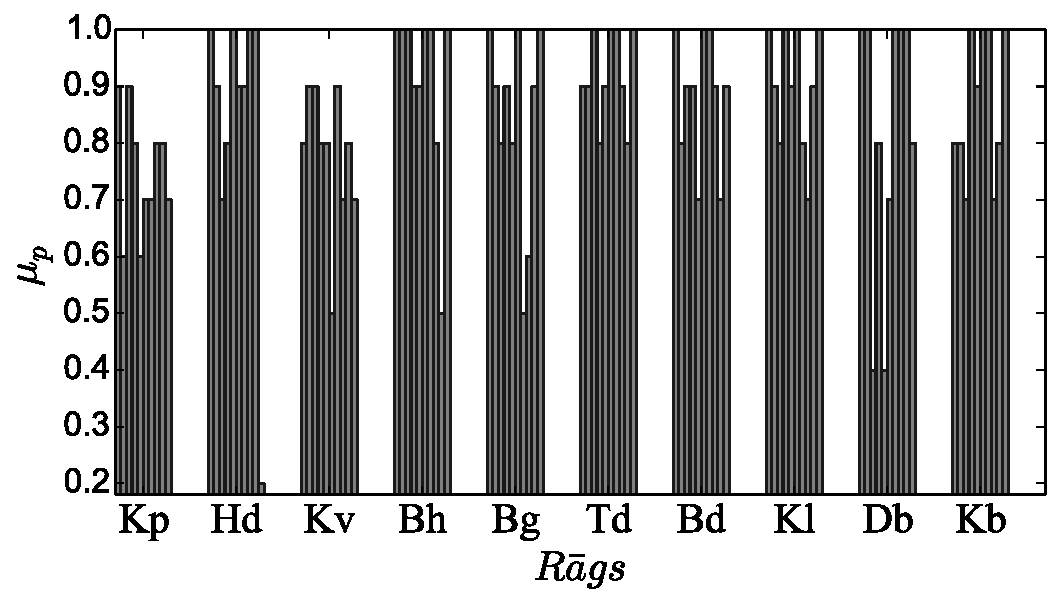
\includegraphics[width=0.88\columnwidth]{figures/per_raaga_per_phrase_rating.pdf}\vSqueezeBig
%	\end{center}
%	\caption{Mean musician rating per melodic phrase for each r\={a}ga: K\={a}pi\,(Kp), Hamsadhvani\,(Hd), K\={a}mavardhini\,(Kv), Bhairavi\,(Bh), Beh\={a}g\,(Bg), T\={o}\d{d}i\,(Td), B\={e}ga\d{d}\={a}\,(Bd), Kaly\={a}\d{n}\={i}\,(Kl), Darb\={a}r\,(Db), K\={a}mb\={o}ji\,(Kb).}\vSqueezeNormal
%	\label{fig:average_rating}
%\end{figure}


We now proceed to analyze the results for different r\={a}gas. In Table~\ref{tab:results_per_raaga}, we summarize mean $\mu_r$ and standard deviation $\sigma_r$ of $\mu_p$ for each r\={a}ga. We observe that there is a considerable amount of variation in $\mu_r$ across the r\={a}gas. It ranges from 0.75 for r\={a}ga K\={a}pi to 0.92 in the case of r\={a}ga T\={o}\d{d}i. An interesting observation here is that the phrase-based r\={a}gas\footnote{R\={a}gas whose identity is derived based on phraseology than svaras~\cite{krishna2012carnatic}.} are the top performing r\={a}gas with the  exception of r\={a}ga Darb\={a}r. From Table~\ref{tab:results_per_raaga} and Table~\ref{tab:dataset_details}, we notice a strong correlation between $\mu_r$ and the total duration of the audio recordings across r\={a}gas. This suggests that longer music pieces are likely to facilitate the discovery of r\={a}ga motifs owing to more number of occurrences of such melodic phrases.

We now examine the melodic phrases with low scores. An investigation of 9 out of 100 phrases that obtain $\mu_p\leq0.6$ reveals that many of these phrases are composition-specific phrases that do not characterize the r\={a}ga. The method wrongly identifies them as r\={a}ga motifs because their associated communities have a high $\gamma$ score owing to a high $\lambda$ value. This can be attributed to the fact that these phrases are discovered from multiple recordings, since their corresponding compositions have several instances in the dataset.  This suggests that, possibly, the goodness measure $\gamma$ can be made more robust to such cases by computing $\lambda$ using the distribution of nodes over unique compositions rather than over audio recordings.

The results show that the proposed method successfully discovers r\={a}ga motifs with a high accuracy. We see that, even for the allied r\={a}gas present in the dataset such as K\={a}mb\={o}ji and B\={e}gada (Section~\ref{sec:music_collection}), the method is able to discover distinct characteristic r\={a}ga motifs. As mentioned, allied r\={a}gas are challenging because they have a substantial overlap in the set of svaras that they comprise (see also Table~\ref{tab:dataset_details}). Finally, on a more informal side, it is worth mentioning that musicians were impressed when, after the listening test, they came to know that the melodic phrases were discovered by a machine following an unsupervised approach. 




%
%\begin{figure}
%	\begin{center}
%		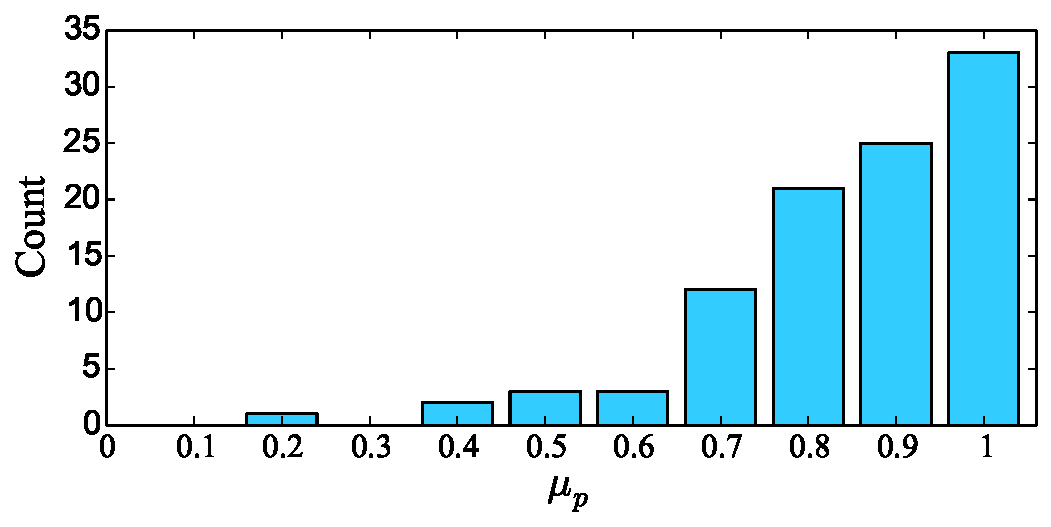
\includegraphics[width=.9\columnwidth]{figures/histogram_musician_rating.pdf}\vSqueezeBig
%	\end{center}
%	\caption{Histogram of $\mu_p$ for all 100 melodic phrases.}\vSqueezeNormal
%	\label{fig:average_rating_histogram}
%\end{figure}

\begin{table} 
	%\tabcolsep = 0.1cm
	\centering
	\begin{tabular}{ l  c c| l | c c }
		\hline\hline
		\multicolumn{1}{ l|  }{R\={a}ga}   			& 	$\mu_r$ 	&	$\sigma_r$	&R\={a}ga   			& 	$\mu_r$ 	&	$\sigma_r$\\	
		\hline
		\multicolumn{1}{ l|  }{Hamsadhvani} 			& 	0.84 		&	0.23 & {\bf B\={e}ga\d{d}a}   	& 	0.88 		&	0.11	\\
		\multicolumn{1}{ l|  }{K\={a}mavardhini} 	& 	0.78 		&	0.17 & K\={a}pi   			& 	0.75 		&	0.10\\	
		\multicolumn{1}{ l|  }{Darb\={a}r}   		& 	0.81 		&	0.23 & {\bf Bhairavi}   			& 	0.91 		&	0.15\\	
		\multicolumn{1}{ l|  }{\bf Kaly\={a}\d{n}i}  & 	0.90 		&	0.10 & Beh\={a}g   		& 	0.84 		&	0.16\\	
		\multicolumn{1}{ l|  }{\bf K\={a}mb\={o}ji}   	& 	0.87 	&	0.12 & {\bf T\={o}\d{d}i}   		& 	0.92 		&	0.07\\	
		\hline\hline
		%   			& 				& 		& 	Overall&0.85 		&	0.16\\ \cline{4-6}\cline{4-6}
		%\hline\hline 
	\end{tabular}
	\caption{Mean $\mu_r$ and standard deviation $\sigma_r$ of $\mu_p$ for each r\={a}ga. R\={a}gas with $\mu_r \geq 0.85$ are highlighted. }
	\label{tab:results_per_raaga}
\end{table}


\section{Conclusion and Future Work}
\label{sec:conclusion}

We presented a novel unsupervised approach to discover r\={a}ga motifs from polyphonic audio music collections of IAM and, specifically, to distinguish them from gamaka and composition-specific motifs. We first extracted melodic patterns from audio recordings using an existing unsupervised approach. We then employed a network analysis and non-overlapping community detection algorithm to cluster melodic patterns. Using the topological properties of the network, we determined a musically meaningful similarity threshold. In addition, we devised a goodness measure for characterizing the detected communities. We evaluated our method using a sizable and representative music collection. A listening test with 10 professional Carnatic musicians shows that the proposed method successfully discovers r\={a}ga motifs with accuracy, even in the presence of allied r\={a}gas in the dataset. This suggests that the functional roles of different melodic phrases in IAM can be effectively exploited to identify them in an unsupervised manner. This, to the best of our knowledge, has been done for the first time in this study. In the future, we plan to extend this work to identify other melodic phrase categories such as composition-specific motifs. Furthermore, we plan to quantitatively evaluate the discovered melodic phrases by using them in tasks such as r\={a}ga recognition and composition identification.


